\chapter{Estados coherentes de la luz. Operadores de compresión y desplazamiento}

\section{Estados número}

% Here I should add the analogy of the QHO with the number states of light, explaining why:
% - n energy value = n number of photons
% - anihilation and creation operators can be used in this states
% - why is the state of number of photons equivalent to the  energy eigenstate

Los valores esperados de los observables, que son representados por operadores Hermitianos en MC, representan las cantidades medibles de un sistema. El campo electromagnético puede ser representado por un espacio de estados, cuantizando un sistema de bosones de masa finita, llamada espacio de Fock. Los estados Fock o número $\ket{n}$ tienen una cantidad definida de número de fotones. El observable que opera sobre los estados Fock es el operador número $\hat{n}_{k\lambda}$, el cual se conforma de los operadores de un solo modo $\hat{a}_{k\lambda}$ y $\hat{a}^{\dagger}_{k\lambda}$. De este punto en adelante, se tratarán a estos operadores para un solo modo, por lo que el subíndice de polarización y modo se omiten y $\hat{n}$, $\hat{a}$ y $\hat{a}^{\dagger}$ corresponderán al operador número, aniquilación y creación de un solo modo de luz.

%Answer the question: What is a mode?: A mode refers to an eigenvector of a linear equation. Consider the coupled springs problem 

Un modo se refiere a un eigenvector de una ecuación de eigenvalores dada. En este caso, si un estado $\ket{\psi}$ es un observable y bajo cierto operador $\mathbf{O}$ genera el mismo estado multiplicado por un eigenvalor $\alpha$, es decir $\mathbf{O}\ket{\psi} = \alpha \ket{\psi}$ decimos que $\ket{\psi}$ es un modo normal (o estado estacionario) del sistema.
Se define al operador número $n$ a partir de los operadores escalera $\hat{n} = \hat{a}^{\dagger}\hat{a}$ y es un operador Hermitiano. Cumple con la ecuación de eigenvalores % Sakurai
\begin{equation*}
  \hat{n}\ket{n} = n \ket{n}
\end{equation*}

Un modo es una onda plana con una polarización dada \cite{Agarwal_2012}. Es un grado de libertad del campo electromagnético donde $n$ es en este caso particular, el número de fotones \cite{Leonhardt}. Los operadores de aniquilación y creación siguen la relación de comutación bosónica

\begin{equation*}
  [\hat{a}, \hat{a}^{\dagger}] = 1
\end{equation*}

y al igual que en el caso del oscilador armónico, se tiene un nivel mínimo de energía, en este caso corresponde al estado vacío $\ket{0}$, es decir, sin \textit{quantum} en el campo de radiación. La definición de los operadores escalera difiere de aquella dada en el oscilador armónico simple, puesto que ahora no se está tratando con partículas con masa. En términos de los operadores posición $\hat{q}$ y momento $\hat{p}$ se definen los operadores de aniquilación y creación como
\begin{equation}\label{eq:crea-anni-def}
  \hat{a} = (2\hbar)^{-1/2}(\hat{q} + i\hat{p}) \quad \hat{a}^{\dagger} = (2\hbar)^{-1/2}(\hat{q} - i\hat{p})
\end{equation} % Perelomov
Cumple con la propiedad $\hat{a} \ket{0} = 0$. La energía en este caso difiere del resultado clásico, ya que $\langle 0\vert\hat{H}\vert 0\rangle = \hbar\omega/2$ con $\omega$ la frecuencia angular correspondiente a ese modo, y esto corresonde a la energía del vacío o energía de punto cero. \cite{Walls} El estado de un fotón se obtiene a partir de este y resulta ser $\ket{1} = \hat{a}^{\dagger} \ket{0}$, y siguiendo este proceso de forma iterativa $n$ veces se obtiene el estado $\ket{n}$ que resulta ser
\begin{equation*}
  \ket{n} = \frac{\hat{a}^{\dagger}}{\sqrt{n!}}\ket{0}
\end{equation*}

Los estados número son ortogonales y completos
\begin{equation*}
  \braket{n_k}{m_k} = \delta_{mn} \quad \sum_{n_k = 0}^{\infty} \ket{n_k} \bra{n_k} = 1
\end{equation*}

La mayoría de los campos ópticos son una superposición de estados número (ensemble puro) o una mezcla de ellos (estado mixto).

% Difference of mixed and pure states: https://physics.stackexchange.com/questions/80434/how-is-a-quantum-superposition-different-from-a-mixed-state

% Mixed state: The ensemble has different types of kets
% Pure state: Superposition of the same type of kets, described by a single ket

\iffalse
  donde se considera la aportación de la energía del vacío. Usando la relación de conmutación de $\hat{a}$ y $\hat{a}^{\dagger}$ sobre el estado vacío $(\hat{a}\hat{a}^{\dagger}-\hat{a}^{\dagger}\hat{a})\ket{0} = \hat{a}\hat{a}^{\dagger}\ket{0} = \ket{0}$ implica que $\hat{a}^{\dagger}\hat{a}(\hat{a}^{\dagger}\ket{0}) = \hat{a}^{\dagger}\ket{0}$, por lo que $\hat{a}^{\dagger}\ket{0}$ es un eigenestado de $\hat{a}^{\dagger}\hat{a}$ con valor propio 1, a este estado se le denomina estado de un fotón y se denota como $\ket{1} = \hat{a}^{\dagger}\ket{0}$. De forma análoga, se puede obtener el n-ésimo estado de $n$ fotones $\ket{n}$ de forma inductiva, lo que resulta en
  \begin{equation*}
    \ket{n} = \frac{\hat{a}^{\dagger\,n}}{\sqrt{n!}}\ket{0}
  \end{equation*}
\fi
% Estados coherentes
\section{Estados coherentes}

% To do - First talk about quadrature of the fields and phasor diagrams
El valor esperado de el operador de aniquilación $\hat{a}$ y los de cuadratura $\hat{X}$ y $\hat{Y}$ son cero, por lo que no tienen una amplitud bien definida de manera clásica. Por otro lado, el haz de un láser es coherente y tiene definida una amplitud y fase. Los estados que representan este fenómeno son los estados coherentes.

Los estados coherentes son el equivalente a un haz monocromático de luz en la mecánica cuántica en el sentido de que son estados de mínima incertidumbre.  Paquetes de onda coherentes derivados del OAC fueron estudiados primeramente por Shcrödinger en 1926, y estos inspiraron el trabajo de Roy J. Glauber \cite{Glauber} que introdujo los estados coherentes (también llamados de Glauber) publicado en 1963 y por el cuál ganó el premio Nobel en 2005. La luz de un láser tiene una amplitud definida, y los estados coherentes $\alpha$ se definen como eigenestados del operador amplitud o aniquilación $\hat{a}$ \cite{Leonhardt}
\begin{equation*}
  \hat{a} \ket{\alpha} = \alpha\ket{\alpha}
\end{equation*}
donde $\alpha$ es en general un número complejo adimensional

El significado físico de $\alpha$ se da considerando un modo polarizado de frecuencia angular $\omega$ dentro de una cavidad de volumen $V$. Se puede definir a $\alpha$ en términos de los valores esperados adimensionales de los operadores de cuadratura
\begin{equation*}
  \alpha = X^2 + iY^2
\end{equation*}
Se puede separar $\alpha$ en su amplitud $|\alpha|=\sqrt{X^2 + Y^2}$ y fase $\phi$ considerando $X = |\alpha|\cos\phi$ y $Y=|\alpha|\sen\phi$ como
\begin{equation*}
  \alpha = |\alpha|e^{i\phi}
\end{equation*}
el estado coherente entonces se puede representar de forma fasorial con longitud $|\alpha|$ y en un ángulo $\phi$.


\begin{figure}[!h]
  \centering
  \tikzset{every picture/.style={line width=0.75pt}} %set default line width to 0.75pt        

  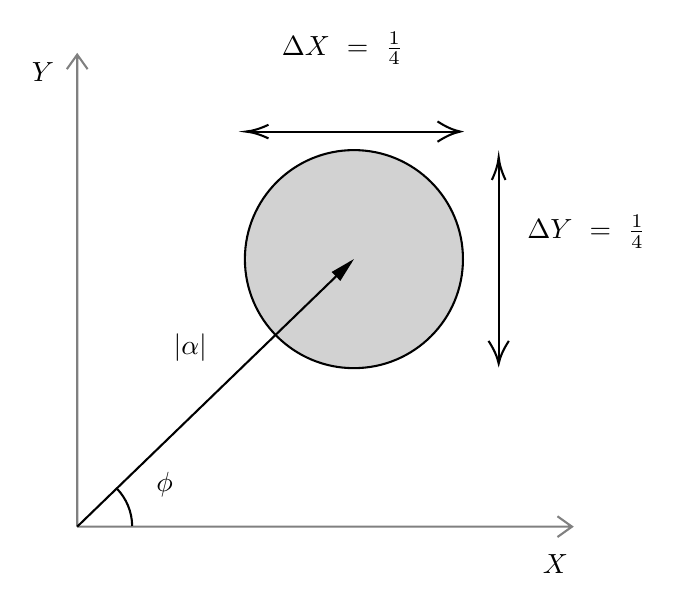
\begin{tikzpicture}[x=0.75pt,y=0.75pt,yscale=-1,xscale=1]
    %uncomment if require: \path (0,475); %set diagram left start at 0, and has height of 475

    %Shape: Axis 2D [id:dp8311178578556598] 
    \draw [color={rgb, 255:red, 128; green, 128; blue, 128 }  ,draw opacity=1 ] (216.09,345.39) -- (454.47,345.39)(216.09,117.96) -- (216.09,345.39) -- cycle (447.47,340.39) -- (454.47,345.39) -- (447.47,350.39) (211.09,124.96) -- (216.09,117.96) -- (221.09,124.96)  ;
    %Shape: Ellipse [id:dp3350713244736996] 
    \draw  [color={rgb, 255:red, 0; green, 0; blue, 0 }  ,draw opacity=1 ][fill={rgb, 255:red, 210; green, 210; blue, 210 }  ,fill opacity=1 ] (296.87,216.49) .. controls (296.87,187.48) and (320.39,163.96) .. (349.4,163.96) .. controls (378.42,163.96) and (401.94,187.48) .. (401.94,216.49) .. controls (401.94,245.5) and (378.42,269.02) .. (349.4,269.02) .. controls (320.39,269.02) and (296.87,245.5) .. (296.87,216.49) -- cycle ;
    %Straight Lines [id:da40847996569793454] 
    \draw    (216.09,345.39) -- (347.97,217.88) ;
    \draw [shift={(349.4,216.49)}, rotate = 135.96] [fill={rgb, 255:red, 0; green, 0; blue, 0 }  ][line width=0.08]  [draw opacity=0] (12,-3) -- (0,0) -- (12,3) -- cycle    ;
    %Straight Lines [id:da07593684349516794] 
    \draw    (299.31,155.04) -- (398.61,155.04) ;
    \draw [shift={(400.61,155.04)}, rotate = 180] [color={rgb, 255:red, 0; green, 0; blue, 0 }  ][line width=0.75]    (10.93,-4.9) .. controls (6.95,-2.3) and (3.31,-0.67) .. (0,0) .. controls (3.31,0.67) and (6.95,2.3) .. (10.93,4.9)   ;
    \draw [shift={(297.31,155.04)}, rotate = 0] [color={rgb, 255:red, 0; green, 0; blue, 0 }  ][line width=0.75]    (10.93,-3.29) .. controls (6.95,-1.4) and (3.31,-0.3) .. (0,0) .. controls (3.31,0.3) and (6.95,1.4) .. (10.93,3.29)   ;
    %Straight Lines [id:da4746690115561758] 
    \draw    (419.15,169.4) -- (419.15,264.82) ;
    \draw [shift={(419.15,266.82)}, rotate = 270] [color={rgb, 255:red, 0; green, 0; blue, 0 }  ][line width=0.75]    (10.93,-4.9) .. controls (6.95,-2.3) and (3.31,-0.67) .. (0,0) .. controls (3.31,0.67) and (6.95,2.3) .. (10.93,4.9)   ;
    \draw [shift={(419.15,167.4)}, rotate = 90] [color={rgb, 255:red, 0; green, 0; blue, 0 }  ][line width=0.75]    (10.93,-3.29) .. controls (6.95,-1.4) and (3.31,-0.3) .. (0,0) .. controls (3.31,0.3) and (6.95,1.4) .. (10.93,3.29)   ;
    %Shape: Arc [id:dp7995525646272961] 
    \draw  [draw opacity=0] (235.25,327.1) .. controls (239.71,331.78) and (242.48,338.09) .. (242.57,345.05) -- (216.09,345.39) -- cycle ; \draw   (235.25,327.1) .. controls (239.71,331.78) and (242.48,338.09) .. (242.57,345.05) ;

    % Text Node
    \draw (313.17,105.48) node [anchor=north west][inner sep=0.75pt]    {$\Delta X\ =\ \frac{1}{4}$};
    % Text Node
    \draw (431.47,193.77) node [anchor=north west][inner sep=0.75pt]    {$\Delta Y\ =\ \frac{1}{4}$};
    % Text Node
    \draw (261.06,250.74) node [anchor=north west][inner sep=0.75pt]    {$|\alpha |$};
    % Text Node
    \draw (252.76,317.84) node [anchor=north west][inner sep=0.75pt]    {$\phi $};
    % Text Node
    \draw (192.72,120.07) node [anchor=north west][inner sep=0.75pt]    {$Y$};
    % Text Node
    \draw (438.99,357.57) node [anchor=north west][inner sep=0.75pt]    {$X$};

  \end{tikzpicture}

  \caption{Estado coherente $\vert \alpha \rangle = \hat{D}(\alpha)\vert 0 \rangle$ con $\phi$ el argumento del parámetro de compresión}
  \label{fig:displaced-vacuum}
\end{figure}


Las cuadraturas están sujetas a la misma incertidumbre que la posición y el momento generalizado del oscilador armónico simple
\begin{equation*}
  \Delta X \Delta Y \geq \frac{1}{4}
\end{equation*}
dado que no hay preferencia entre las dos cuadraturas, se concluye que sus incertidumbres son iguales
\begin{equation*}
  \Delta X = \Delta Y = \frac{1}{2}
\end{equation*}
Por ser $\hat{a}$ no Hermitiano, los eigenvalores de los estados coherentes son complejos, y estos corresponden físicamente a las amplitudes de onda complejas en óptica clásica, con magnitud $|\alpha|$ y fase $\arg \alpha$. El estado cuántico de un haz láser continuo es un ensemble de estados coherentes con fase aleatoria.

El estado vacío es un estado coherente, ya que satisface la ecuación $\hat{a} \ket{0} = 0 \ket{0} = 0$, y corresponde a un estado de amplitud cero. La energía promedio de un estado coherente corresponde a
\begin{equation*}
  \langle \alpha \vert \hat{H}\vert \alpha \rangle = \left\langle \alpha \right\vert \hat{a}^{\dagger}\hat{a} + \frac{1}{2} \left\vert \alpha \right\rangle = |\alpha|^2 + \frac{1}{2}
\end{equation*}

El valor esperado del operador de aniquilación (o también llamado amplitud) $\hat{a}$, y las cuadraturas, bajo los estados coherentes ahora ti tienen un amplitud definida.
\begin{equation*}
  \langle \alpha \vert \hat{a} \vert\alpha \rangle = \alpha \quad \langle \alpha \vert \hat{X} \vert \alpha \rangle = \frac{\mathrm{Re}\alpha}{\sqrt{2}} \quad \langle \alpha \vert \hat{Y} \vert \alpha\rangle = \frac{\mathrm{Im}\alpha}{\sqrt{2}}
\end{equation*}
(Figura de distribución de fotones Agarwal)
Los estados coherentes se pueden descomponer en una suma de estados número
\begin{equation*}
  \ket{\alpha} = \sum_{n=0}^{\infty} c_n \ket{n}
\end{equation*}
Los coeficientes se calculan a partir de la relación de recursión
\begin{equation*}
  c_{n+1} = \frac{\alpha}{\sqrt{n+1}}c_n
\end{equation*}
y resultan
\begin{equation*}
  c_n = \frac{\alpha^n }{\sqrt{n!}}c_0
\end{equation*}
El valor de $c_0$ se puede encontrar a partir de la condición de normalización, como los estados número son ortonormales, se obtiene
\begin{align*}
  1 = \braket{\alpha}{\alpha} & = c_0^2 \sum_{n=0}^{\infty} \frac{(\alpha^n)^2}{(\sqrt{n!})^2}\braket{n}{n} \\ &= c_0^2  \sum_{n=0}^{\infty} \frac{(|\alpha|^2)^2}{n!}\braket{n}{n}\\ &= c_0^2 e^{|\alpha|^2} \\
  c_0                         & = e^{-\frac{1}{2}|\alpha|^2}
\end{align*}
y la superposición de estados número resulta de manera explícita
\begin{equation*}
  \ket{\alpha} = e^{-\frac{1}{2}|\alpha|^2} \sum_{n=0}^{\infty} \frac{\alpha^n}{\sqrt{n!}}\ket{n}
\end{equation*}
La probabilidad de encontrar $n$ fotones en estado coherente se da por una distribución de Poisson con media $|\alpha|^2$, y esta es a su vez igual a la varianza $\langle n \rangle = |\alpha|^2 = \langle n^2 \rangle = \langle n \rangle^2$.

Los estados coherentes forman una base sobrecompleta, es decir, son completos pero no son ortonormales entre sí. La condición de completez es
\begin{equation*}
  \frac{1}{\pi}\int d^2 \alpha \ket{\alpha}\bra{\alpha} = 1
\end{equation*}
donde $\alpha$ es un número complejo y la integral se realiza sobre el plano complejo, siendo $d^2\alpha = dxdy$, con $x = \mathrm{Re}\alpha$ y $y = \mathrm{Im}\alpha$. La desmostración se da sustituyendo la definición de $\ket{\alpha}$ en la condición de completez y verificando que $\sum_n \ket{\alpha}\bra{\alpha}=1$. sustituyendo en el lado izquierdo
\begin{equation*}
  \sum_{n.m} \frac{1}{\sqrt{n!m!}}\int d^2\alpha (\alpha)^n \alpha^{*m}\ket{n}\bra{m}e^{-|\alpha|^2}
\end{equation*}
que cambiando a coordenadas polares
\begin{align*}
  1 & = \sum_{n,m}\frac{1}{\sqrt{n!m!}}\int_0^{\infty} rdr \int_{0}^{2\pi}d\theta (r)^{n+m}e^{i\theta(n-m)}\ket{n}\bra{m}e^{-r^2} \\ & = \sum_{n,m}\frac{1}{\sqrt{n!m!}}\int_0^{\infty} rdr  (r)^{n+m} \delta_{nm} \ket{n}\bra{m}e^{-r^2} \\
    & = \sum_{n}\frac{1}{n!}\int_0^{\infty} dr  r^{2n+1} \ket{n}\bra{n}e^{-r^2}                                                   \\
    & = \sum_{n} \ket{n}\bra{n} \frac{1}{n!}\int_0^{\infty} dr  r^{2(n+1)-1} e^{-r^2}                                             \\
    & = \sum_{n} \ket{n}\bra{n} \frac{1}{n!} \Gamma(n+1)                                                                          \\
  1 & = \sum_{n} \ket{n}\bra{n}
\end{align*}
La sobrecompletitud hace que los estados sean no ortogonales entre si, el producto interno entre dos elementos del espacio de estados coherentes es distinto de cero, y es en particular se puede calcular de la expresión de estado coherente
\begin{align*}
  \braket{\alpha|\beta} & = e^{-\frac{1}{2}|\alpha|^2} e^{-\frac{1}{2}|\beta|^2} \sum_{n,m=0}^{\infty} \frac{{\alpha^*}^n}{\sqrt{n!}}\frac{\beta^m}{\sqrt{m!}} \braket{n}{m} \\
                        & = e^{-\frac{1}{2}|\alpha|^2} e^{-\frac{1}{2}|\beta|^2} \sum_{n=0}^{\infty} \frac{{(\alpha^*\beta)}^n}{n!} \braket{n}{n}                            \\
                        & = \exp{\left( - \frac{1}{2}|\alpha|^2 - \frac{1}{2}|\beta|^2 + \alpha^*\beta \right)}
\end{align*}
De lo anterior, un estado coherente se puede escribir en términos de otros estados coherentes. Considerando el braket de un par de estados coherentes $\ket{\alpha}$ y $\ket{\gamma}$, y utilizando la condición de completez
\begin{align*}
  \braket{\alpha|\gamma}             & =  \bra{{\alpha}}\left(\frac{1}{\pi}\int d^2 \alpha \ket{\beta}\bra{\beta} \right) \ket{\gamma}      \\
                                     & = \left(\frac{1}{\pi}\int d^2 \beta \braket{\alpha}{\beta}\braket{\beta}{\gamma} \right)             \\
  \frac{\braket{\alpha|\gamma}}{\pi} & = \left(\int d^2 \beta \frac{\braket{\alpha}{\beta}}{\pi} \frac{\braket{\beta}{\gamma}}{\pi} \right)
\end{align*}
Escrito de esta forma, podemos ver que $\frac{\braket{\alpha}{\beta}}{\pi}$ es un núcleo reproductor denotado por $K(\alpha, \beta)$, que proviene de la no-ortogonalidad de los estados coherentes. Se puede entonces reescribir lo anterior como
\begin{equation*}
  K(\alpha, \gamma) = \int d^2 \beta K(\alpha, \beta) K(\beta, \gamma)
\end{equation*}
Así, de nuevo por la condición de completez, podemos escribir cualquier estado coherente $\ket{\alpha}$ en términos de otro $\ket{\beta}$
\begin{equation*}
  \ket{\alpha} = \int K(\alpha, \beta) \ket{\beta} d^2\beta
\end{equation*}
% Grupo y álgebra de Heisenberg Weyl
\section{Grupos y Álgebras de Lie, Grupo de Heisenberg-Weyl}

El teorema de Noether estipula que correspondiente a cada ley de conservación existe una simetría diferenciable. En particular establece una conexión entre el generador de una transformación de simetría con la cantidad conservada. El estudio de estas cantidades conservadas es la base de la física, pues describen a los sistemas en sí. En la mecánica cuántica se puede ver como generador de traslaciones en el espacio $-i\delta_i$ al momento $\hat{p}_i$, mientras que la energía $\hat{E}$ como cantidad conservada proviene de la invarianza bajo la acción del generador de traslaciones temporales $i\delta_0$. La posición no tiene relacionada una simetría o ley de conservación, por lo que simplemente se utiliza el operador de posición $\hat{x}_i$. \cite{Schwichtenberg}

Las cantidades físicas de la teoría son representadas por operadores diferenciales. Para entender a detalle cómo funcionan los operadores, sobre qué actúan y cómo se relacionan a cantidades físicas medibles primero se tiene que estudiar las simetrías, que son la invarianza bajo alguna transformación y que es el objeto de estudio de la teoría de grupos. El grupo de Poincaré es el conjunto de todas las transformaciones permitidas por estas restricciones, donde el objeto invariante es la métrica de Minkowski en el espacio-tiempo.

Un grupo es una colección de transformaciones. Formalmente es un conjunto $G$ con una operación binaria $\circ$ de finida en $G$ que satisface cuatro condiciones
\begin{enumerate}
  \item Sean $g_1,g_2 \in G$ dos elementos del grupo, entonces el producto de $g_1$ y $g_2$ bajo $\circ$ pertenece también al grupo, es decir $g_1 \circ g_2 \in G$.
  \item Existe un elemento $e\in G$ tal que para toda $g\in G$, $g\circ g = g$. A este elemento se le llama identidad.
  \item Para cada $g\in G$ existe un elemento $g^{-1}$ llamado inverso que cumple $g\circ g^{-1} = g^{-1}\circ g =e$
  \item Asociatividad. Para todo $g_1, g_2, g_3 \in G$, $g_1 \circ (g_2 \circ g_3) = (g_1 \circ g_2) \circ g_3$
\end{enumerate}

Las transformaciones bajo las cuales se conserva una simetría pueden ser continuas o discretas. Considere el caso de una rotación de un cuadrado centrado en $x,y=0$ en el plano cartesiano. Matemáticamente un cuadrado es un conjunto de puntos, y su simetría es una transformación que  Al rotar el cuadrado por una cantidad menor de $pi/2$ radianes en dirección contrarreloj respecto al origen sobre el plano $xy$, las nuevas posiciones de los vértices no coinciden con las posiciones de estos previo a la rotación. Sin embargo, cuando se hace una rotación de $n\pi/2$ radianes con $n\in \mathbb{Z}$, los vértices se alinearán con las posiciones iniciales, y bajo esta transformación es virtualmente imposible diferenciar entre el cuadrado previo o posterior a esta. Se dice entonces que el sistema es simétrico ante rotaciones discretas de $n\pi/2$ radianes.


\begin{figure}[!h]
  \centering
  \tikzset{every picture/.style={line width=0.75pt}} %set default line width to 0.75pt        

  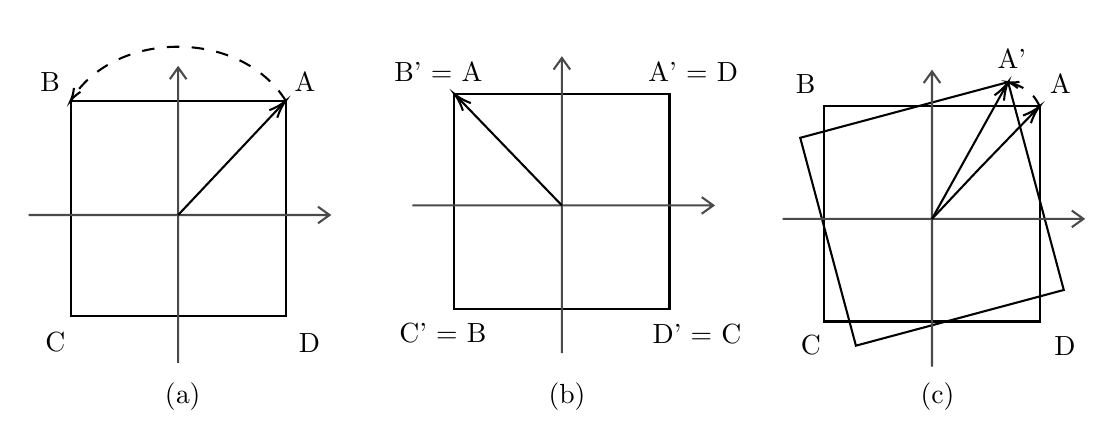
\begin{tikzpicture}[x=0.6pt,y=0.6pt,yscale=-1,xscale=1]
    %uncomment if require: \path (0,476); %set diagram left start at 0, and has height of 476

    %Shape: Square [id:dp022247054189771465] 
    \draw  [color={rgb, 255:red, 0; green, 0; blue, 0 }  ,draw opacity=1 ][line width=0.75]  (476.44,155.98) -- (601.62,122.44) -- (635.16,247.62) -- (509.98,281.16) -- cycle ;
    %Shape: Square [id:dp42752261729009344] 
    \draw  [color={rgb, 255:red, 0; green, 0; blue, 0 }  ,draw opacity=1 ] (491,137) -- (620.6,137) -- (620.6,266.6) -- (491,266.6) -- cycle ;
    %Shape: Axis 2D [id:dp33838415100218366] 
    \draw [color={rgb, 255:red, 74; green, 74; blue, 74 }  ,draw opacity=1 ] (465.8,204.8) -- (647,204.8)(555.8,116) -- (555.8,293.8) (640,199.8) -- (647,204.8) -- (640,209.8) (550.8,123) -- (555.8,116) -- (560.8,123)  ;
    %Curve Lines [id:da6325068560094059] 
    \draw [color={rgb, 255:red, 0; green, 0; blue, 0 }  ,draw opacity=1 ] [dash pattern={on 4.5pt off 4.5pt}]  (620.6,137) .. controls (618.07,131.22) and (614,126.25) .. (603.52,122.99) ;
    \draw [shift={(601.62,122.44)}, rotate = 15.25] [color={rgb, 255:red, 0; green, 0; blue, 0 }  ,draw opacity=1 ][line width=0.75]    (6.56,-1.97) .. controls (4.17,-0.84) and (1.99,-0.18) .. (0,0) .. controls (1.99,0.18) and (4.17,0.84) .. (6.56,1.97)   ;
    %Straight Lines [id:da30604344238116343] 
    \draw    (555.8,204.8) -- (584.18,174.67) -- (619.21,138.44) ;
    \draw [shift={(620.6,137)}, rotate = 134.03] [color={rgb, 255:red, 0; green, 0; blue, 0 }  ][line width=0.75]    (10.93,-3.29) .. controls (6.95,-1.4) and (3.31,-0.3) .. (0,0) .. controls (3.31,0.3) and (6.95,1.4) .. (10.93,3.29)   ;
    %Straight Lines [id:da7434943351940627] 
    \draw [color={rgb, 255:red, 0; green, 0; blue, 0 }  ,draw opacity=1 ]   (555.8,204.8) -- (600.65,124.18) ;
    \draw [shift={(601.62,122.44)}, rotate = 119.09] [color={rgb, 255:red, 0; green, 0; blue, 0 }  ,draw opacity=1 ][line width=0.75]    (10.93,-3.29) .. controls (6.95,-1.4) and (3.31,-0.3) .. (0,0) .. controls (3.31,0.3) and (6.95,1.4) .. (10.93,3.29)   ;

    %Shape: Square [id:dp33381188559407793] 
    \draw  [color={rgb, 255:red, 0; green, 0; blue, 0 }  ,draw opacity=1 ] (37,133.67) -- (166.6,133.67) -- (166.6,263.27) -- (37,263.27) -- cycle ;
    %Shape: Axis 2D [id:dp050369217976065195] 
    \draw [color={rgb, 255:red, 74; green, 74; blue, 74 }  ,draw opacity=1 ] (11.8,202.47) -- (193,202.47)(101.8,113.67) -- (101.8,291.47) (186,197.47) -- (193,202.47) -- (186,207.47) (96.8,120.67) -- (101.8,113.67) -- (106.8,120.67)  ;
    %Curve Lines [id:da7677316032904558] 
    \draw  [dash pattern={on 4.5pt off 4.5pt}]  (166.6,133.67) .. controls (139.87,90.71) and (65.12,90.28) .. (37.81,132.39) ;
    \draw [shift={(37,133.67)}, rotate = 301.5] [color={rgb, 255:red, 0; green, 0; blue, 0 }  ][line width=0.75]    (7.65,-2.3) .. controls (4.86,-0.97) and (2.31,-0.21) .. (0,0) .. controls (2.31,0.21) and (4.86,0.98) .. (7.65,2.3)   ;
    %Straight Lines [id:da09676489903078345] 
    \draw    (101.8,202.47) -- (130.18,172.35) -- (165.23,135.13) ;
    \draw [shift={(166.6,133.67)}, rotate = 133.29] [color={rgb, 255:red, 0; green, 0; blue, 0 }  ][line width=0.75]    (10.93,-3.29) .. controls (6.95,-1.4) and (3.31,-0.3) .. (0,0) .. controls (3.31,0.3) and (6.95,1.4) .. (10.93,3.29)   ;

    %Shape: Square [id:dp2056284721834185] 
    \draw  [color={rgb, 255:red, 0; green, 0; blue, 0 }  ,draw opacity=1 ] (268.1,129.5) -- (397.7,129.5) -- (397.7,259.1) -- (268.1,259.1) -- cycle ;
    %Shape: Axis 2D [id:dp6729784801445232] 
    \draw [color={rgb, 255:red, 74; green, 74; blue, 74 }  ,draw opacity=1 ] (242.9,196.7) -- (424.1,196.7)(332.9,107.9) -- (332.9,285.7) (417.1,191.7) -- (424.1,196.7) -- (417.1,201.7) (327.9,114.9) -- (332.9,107.9) -- (337.9,114.9)  ;
    %Straight Lines [id:da5397537113648408] 
    \draw    (332.9,196.7) -- (269.49,130.94) ;
    \draw [shift={(268.1,129.5)}, rotate = 46.04] [color={rgb, 255:red, 0; green, 0; blue, 0 }  ][line width=0.75]    (10.93,-3.29) .. controls (6.95,-1.4) and (3.31,-0.3) .. (0,0) .. controls (3.31,0.3) and (6.95,1.4) .. (10.93,3.29)   ;


    % Text Node
    \draw (170,114.67) node [anchor=north west][inner sep=0.75pt]   [align=left] {A};
    % Text Node
    \draw (17,114.67) node [anchor=north west][inner sep=0.75pt]   [align=left] {B};
    % Text Node
    \draw (20,271.67) node [anchor=north west][inner sep=0.75pt]   [align=left] {C};
    % Text Node
    \draw (172.6,272.27) node [anchor=north west][inner sep=0.75pt]   [align=left] {D};
    % Text Node
    \draw (92,301.5) node [anchor=north west][inner sep=0.75pt]   [align=left] {(a)};
    % Text Node
    \draw (383.1,108.9) node [anchor=north west][inner sep=0.75pt]   [align=left] {A' = D};
    % Text Node
    \draw (230.1,108.9) node [anchor=north west][inner sep=0.75pt]   [align=left] {B' = A};
    % Text Node
    \draw (233.1,265.9) node [anchor=north west][inner sep=0.75pt]   [align=left] {C' = B};
    % Text Node
    \draw (385.7,266.5) node [anchor=north west][inner sep=0.75pt]   [align=left] {D' = C};
    % Text Node
    \draw (323,301.5) node [anchor=north west][inner sep=0.75pt]   [align=left] {(b)};
    % Text Node
    \draw (625,116) node [anchor=north west][inner sep=0.75pt]   [align=left] {A};
    % Text Node
    \draw (472,116) node [anchor=north west][inner sep=0.75pt]   [align=left] {B};
    % Text Node
    \draw (475,273) node [anchor=north west][inner sep=0.75pt]   [align=left] {C};
    % Text Node
    \draw (627.6,273.6) node [anchor=north west][inner sep=0.75pt]   [align=left] {D};
    % Text Node
    \draw (593.4,100.8) node [anchor=north west][inner sep=0.75pt]   [align=left] {A'};
    % Text Node
    \draw (547,301.5) node [anchor=north west][inner sep=0.75pt]   [align=left] {(c)};

  \end{tikzpicture}

  \caption{Rotación de un cuadrado (a) Posición inicial de los vértices (b) Posición final de los vértices tras una rotación de $\frac{\pi}{2}$ rad. (c) Rotación por $5^\circ$ donde los vértices de la posición inicial no coinciden con los de la posición final}
  \label{fig:square-rotation}
\end{figure}


Por otro lado, considere ahora una circunferencia de radio $a$ centrada en $x,y=0$. Rotando sobre el plano $xy$ respecto al origen cualquier cantidad de $\phi$ radianes será imposible distinguir entre la circunferencia rotada y la no transformada. El anterior es un ejemplo de una simetría continua, que es el objeto de estudio del álgebra de Lie.

\begin{figure}[!h]
  \centering

  \tikzset{every picture/.style={line width=0.75pt}} %set default line width to 0.75pt        

  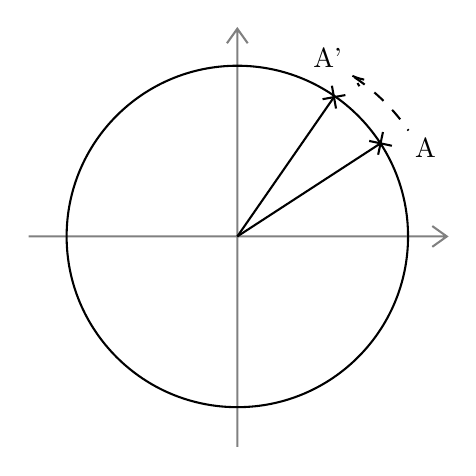
\begin{tikzpicture}[x=0.75pt,y=0.75pt,yscale=-1,xscale=1]
    %uncomment if require: \path (0,473); %set diagram left start at 0, and has height of 473

    %Shape: Axis 2D [id:dp09236434939221472] 
    \draw [color={rgb, 255:red, 128; green, 128; blue, 128 }  ,draw opacity=1 ] (230.16,226.68) -- (431.6,226.68)(330.67,126.6) -- (330.67,328.04) (424.6,221.68) -- (431.6,226.68) -- (424.6,231.68) (325.67,133.6) -- (330.67,126.6) -- (335.67,133.6)  ;
    %Straight Lines [id:da6379035327346838] 
    \draw    (330.67,226.68) -- (399.67,181.83) ;
    \draw [shift={(399.67,181.83)}, rotate = 11.97] [color={rgb, 255:red, 0; green, 0; blue, 0 }  ][line width=0.75]    (-5.59,0) -- (5.59,0)(0,5.59) -- (0,-5.59)   ;
    %Straight Lines [id:da23036927116370676] 
    \draw [color={rgb, 255:red, 0; green, 0; blue, 0 }  ,draw opacity=1 ]   (330.67,226.68) -- (377.23,159.56) ;
    \draw [shift={(377.23,159.56)}, rotate = 349.75] [color={rgb, 255:red, 0; green, 0; blue, 0 }  ,draw opacity=1 ][line width=0.75]    (-5.59,0) -- (5.59,0)(0,5.59) -- (0,-5.59)   ;
    %Shape: Ellipse [id:dp4110738875267169] 
    \draw  [color={rgb, 255:red, 0; green, 0; blue, 0 }  ,draw opacity=1 ] (248.42,226.68) .. controls (248.42,181.26) and (285.24,144.43) .. (330.67,144.43) .. controls (376.1,144.43) and (412.92,181.26) .. (412.92,226.68) .. controls (412.92,272.11) and (376.1,308.94) .. (330.67,308.94) .. controls (285.24,308.94) and (248.42,272.11) .. (248.42,226.68) -- cycle ;
    %Shape: Arc [id:dp6746872257873422] 
    \draw  [draw opacity=0][dash pattern={on 4.5pt off 4.5pt}] (385.33,148.85) .. controls (396.38,155.91) and (405.85,165.04) .. (413.12,175.66) -- (330.67,226.68) -- cycle ; \draw [dash pattern={on 4.5pt off 4.5pt}] [dash pattern={on 4.5pt off 4.5pt}]  (387.14,150.03) .. controls (397.42,156.92) and (406.25,165.62) .. (413.12,175.66) ;  \draw [shift={(385.33,148.85)}, rotate = 36.08] [color={rgb, 255:red, 0; green, 0; blue, 0 }  ][dash pattern={on 4.5pt off 4.5pt}][line width=0.75]    (6.56,-1.97) .. controls (4.17,-0.84) and (1.99,-0.18) .. (0,0) .. controls (1.99,0.18) and (4.17,0.84) .. (6.56,1.97)   ;

    % Text Node
    \draw (414.83,178.25) node [anchor=north west][inner sep=0.75pt]   [align=left] {A};
    % Text Node
    \draw (365.81,134.48) node [anchor=north west][inner sep=0.75pt]   [align=left] {A'};


  \end{tikzpicture}

  \caption{Rotación de un círculo, la simetría es continua y los puntos inicial y final son indistinguibles entre si}
  \label{fig:circle-rotation}
\end{figure}


De manera más formal, sea $\mathbf{a}$ un vector y $O$ una transformación, que mantenga la norma de este, es decir que $|\mathbf{a}| = |O\mathbf{a}|$. La transformación tiene que ser ortogonal, es decir $O^{T}O = I$. Las transformaciones ortogonales en dos dimensiones se denotan por $O(2)$. Estas transformación también cumplen $\det(O) = \pm 1$, esta característica les da el nombre de grupo especial ortogonal, y se denota por $SO(2)$. Una matriz de rotación en dos dimensiones por un ángulo $\theta$ se representa matricialmente como
\begin{equation*}
  R_\theta = \begin{pmatrix}
    \cos(\theta) & -\sen(\theta) \\
    \sen(\theta) & cos(\theta)
  \end{pmatrix}
\end{equation*}

Por otro lado, los números complejos junto a su operación de multiplicación forman un grupo unitario llamado $U(1)$, el cuál se caracteriza por la condición $U^\dagger U = 1$. La transformación se escribe usando el parámetro $\theta$ como
\begin{equation*}
  R_\theta = e^{i\theta} = \cos(\theta) + i\sen(\theta)
\end{equation*}
que cumple la característica de ser unitaria.

Las anteriores dos transformaciones describen rotaciones, y son un ejemplo de dos representaciones que actuan de la misma manera, formando un isomorfismo entre $SO(2)$ y $U(1)$. La representación matricial de los números complejos es entonces
\begin{equation*}
  1 = \begin{pmatrix}
    1 & 0 \\ 0 & 1
  \end{pmatrix} \quad i = \begin{pmatrix}
    0 & -1 \\ 1 & 0
  \end{pmatrix}
\end{equation*}
Para el caso de la circunferencia, se puede realizar una rotación con un argumento tan pequeño como se guste, una rotación arbitrariamente cercana a la identidad, a diferencia de los grupos discretos  donde el parámetro de transformación no es continuo y por tanto no hay elementos arbitrariamente cercanos a la identidad. Esta transformación infinitesimal se define como
\begin{equation*}
  g(\epsilon) = I + gX
\end{equation*}
donde $\epsilon>0$ es un número pequeño y $X$ es un objeto llamado generador. Una transformación infinitesimal aplicada de manera sucesiva genera una transformación finita $h(\theta) = \prod_k (I+\epsilon X)$, con $\theta$ un parámetro de transformación finita. Se puede reescribir $\epsilon$ en términos del parámetro de transformación finita $\theta$ dividiendo este último entre un número entero arbitrariamente grande $N$. El generador es entonces
\begin{equation*}
  g(\theta) = I = \frac{\theta}{N} X
\end{equation*}
Aplicando esta transformación $N$ veces, y aplicando el límite $N\to\infty$ se genera una transformación finita
\begin{equation*}
  h(\theta) = \lim_{N\to\infty}\left( I + \frac{\theta}{N}X \right)^N = e^{\theta X}
\end{equation*}
observamos entonces que la transformación de argumento finito $\theta$ es generada por $X$. Para calcular el generador se obtiene la derivada de la transformación finita respecto al argumento y se evalúa en $\theta=0$
\begin{equation}\label{eq:generator}
  X = \frac{dh(\theta)}{d\theta} \bigg|_{\theta=0}
\end{equation}
los generadores brindan información importante sobre los grupos que se estudian.
En el caso particular de un grupo de transformaciones dado por matrices, se puede calcular la expansión en series de Taylor de un elemento del grupo cercano a la identidad
\begin{equation*}
  h(\theta) = I + \frac{dh}{d\theta}\bigg|_{\theta=0}\theta + \frac{1}{2}\frac{d^2h}{d\theta^2}\bigg|_{\theta=0}\theta^2 + \dots = \sum_{n=0}^{\infty} \frac{1}{n!}\frac{d^n h}{h\theta^n}\bigg|_{\theta=0}\theta^n
\end{equation*}
Para grupos de matrices de Lie se define un correspondiente álgebra de Lie como una colección de objetos que generan un elemento del grupo cuando se calculan sus exponenciales. Para un grupo de Lie $G$ dado por matrices de dimensión $n\times n$, el álgebra $\mathfrak{g}$ de $G$ está dada por aquellas matrices $n\times n$ $X$ tales que $e^{tX}\in G$ para $t\in \mathbb{R}$, junto a una operación llamada corchete de Lie $[,]$ que define cómo se combinan estas matrices. La multiplicación de dos elementos del álgebra de Lie no necesariamente es un elemento de este mismo, es decir, no es cerrada bajo la multiplicación del grupo, pero si lo es bajo el corchete de Lie. La relación entre el álgebra de Lie y el grupo de Lie está dada por la fórmula de Baker-Campbell-Hausdorff
\begin{equation*}
  e^X \circ e^Y = e^{X+Y+\frac{1}{2}[X,Y] + \frac{1}{12}[X,[X,Y]] - \frac{1}{12}[Y,[X,Y]] + \dots}
\end{equation*}
del lado izquierdo, hay dos elementos del grupo escritos en término de los generadores $X,Y\in \mathfrak{g}$, mientras que del lado derecho se tiene un solo elemento del grupo y la multiplicación de elementos del grupo se ha transformado en una suma de elementos del álgebra de Lie. En el caso particular de matrices, el corchete de Lie es el conmutador $[X,Y] = XY-YX$.
De manera formal, un álgebra de Lie es un espacio vectorial $\mathfrak{g}$ junto a una operación binaria $[,]:\mathfrak{g}\times \mathfrak{g} \to \mathfrak{g}$. La operación binaria satisface los siguientes axiomas:
\begin{enumerate}
  \item Bilinearidad: $[aX + bY, Z] = a[X,Y] + b[Y, Z]$ y $[Z, aX + bY] = a[Z,X] + b[Z,Y]$ para $a,b\in \mathbb{F}$ con $\mathbb{F}$ un cuerpo, y se cumple para todo $X,Y,Z\in \mathfrak{g}$
  \item Anti-conmutatividad: $[X,Y] = -[Y,X]$, $\forall X, Y \in \mathfrak{g}$
  \item Satisfacen la identidad de Jacobi: $[X, [Y,Z]] + [Z,[X,Y]] + [Y,[Z,X]] = 0$, $\forall X,Y,Z\in \mathfrak{g}$
\end{enumerate}
Diferentes grupos pueden tener el mismo álgebra de Lie, la diferencia d estos es cómo los generadores de estos grupos se comportan bajo el álgebra de Lie.
Considerando el ejemplo particular de las matrices de rotación $SO(3)$, recordando que estas están dadas por
\begin{equation*}
  R_x = \begin{pmatrix}
    1 & 0            & 0             \\
    0 & \cos(\theta) & -\sen(\theta) \\
    0 & \sen(\theta) & \cos(\theta)
  \end{pmatrix} \quad
  R_y = \begin{pmatrix}
    \cos(\theta)  & -\sen(\theta) & 0            \\
    0             & 1             & 0            \\
    -\sen(\theta) & 0             & \cos(\theta)
  \end{pmatrix}
\end{equation*}
\begin{equation*}
  R_z = \begin{pmatrix}
    \cos(\theta) & -\sen(\theta) & 0 \\
    \sen(\theta) & \cos(\theta)  & 0 \\
    0            & 0             & 1
  \end{pmatrix}
\end{equation*}
Las condiciones de estas transformaciones son las mismas que las rotaciones en dos dimensiones, es decir, son ortogonales $O^T O = I$ y su determinante es la unidad $\det(O) = 1$. Un elemento cualesquiera del grupo en términos de un generador $J$ está dado por $O = e^{\theta J}$. Sustituyendo esto en las condiciones de las transformaciones se obtiene que $J^T + J = 0$ y $\mathrm{Tr}(J) = 0$. A partir de estas condiciones se pueden escribir tres elementos linealmente independientes que formen una base para $SO(3)$, considere
\begin{equation*}
  J_1 = \begin{pmatrix}
    0 & 0 & 0 \\ 0 & 0 & -1 \\ 0 & 1 & 0
  \end{pmatrix} \quad
  J_2 = \begin{pmatrix}
    0 & 0 & 1 \\ 0 & 0 & 0 \\ -1 & 0 & 0
  \end{pmatrix} \quad
  J_3 = \begin{pmatrix}
    0 & -1 & 0 \\ 1 & 0 & 0 \\ 0 & 0 & 0
  \end{pmatrix} \quad
\end{equation*}
Así, cualquier generador se puede escribir de la forma $J = aJ_1+ bJ_2+cJ_3$. Las entradas de las bases se pueden representar por
\begin{equation*}
  (J_i)_{jk} = -\epsilon_{ijk}
\end{equation*}
Como en este caso se conocen de antemano las matrices de rotación, se puede ocupar la fórmula (\ref{eq:generator}) para deducir $J_i$ de cada matriz de rotación $R_i$, para $J_1$ por ejemplo
\begin{equation*}
  J_1 = \frac{dR_1}{d\theta}\bigg|_{\theta=0} = \begin{pmatrix}
    0 & 0 & 0 \\ 0 & -\sen(\theta) & -cos(\theta)\\ 0 & \cos(\theta) & -\sen(\theta)
  \end{pmatrix} \Bigg|_{\theta=0} = \begin{pmatrix}
    0 & 0 & 0 \\ 0&0&-1\\ 0&1&0
  \end{pmatrix}
\end{equation*}
\section{Operador desplazamiento}
Los operadores que se utilizan con frecuencia para describir sistemas cuánticos con un grado de libertad son la posición $\hat{q}$ y momento $\hat{p}$ y tienen las relaciones de conmutación de Heisenberg $[\hat{q}, \hat{p}] = i\hbar \hat{I}$, $[\hat{q}, \hat{I}] = [\hat{p}, \hat{I}]=0$ con $\hat{I}$ el operador identidad. Estos operadores actuan sobre un espacio de Hilbert $\mathcal{H}$. A partir de estos operadores se definieron los operadores escalera $\hat{a}$ y $\hat{a}^{\dagger}$, que siguen las relaciones de conmutación $[\hat{a}, \hat{a}^{\dagger}] = \hat{I}$, $[\hat{a}, \hat{I}]=[\hat{a}^{\dagger}, \hat{I}] = 0$. Estas relaciones de conmutación entre los operadores $\hat{q}$, $\hat{p}$ y la identidad $\hat{I}$ (y respectivamente $\hat{a}$, $\hat{a}^{\dagger}$ y $\hat{I}$) indica que estos son generadores de un álgebra de Lie $\mathcal{W}_1$, a la que se le llama álgebra de Heisenberg-Weyl \cite{Perelomov}. Este álgebra tridimensional se define usando las siguientes cantidades
\begin{equation*}
  e_1 = i\frac{\hat{p}}{\sqrt{\hbar}}, \quad e_2 = i\frac{\hat{q}}{\sqrt{\hbar}}, \quad e_3 = i\hat{I}
\end{equation*}
que, además de ser elementos abstractos del álgebra de Lie, son a su vez operadores en un espacio de Hilbert. Las relaciones de conmutación de este álgebra son
\begin{equation*}
  [e_1, e_2] = e_3, \quad [e_1, e_3] = [e_2, e_3] = 0
\end{equation*}
Un elemento $x$ del álgebra de Lie se representa por una combinación lineal $x = x_1e_1 + x_2e_2 + s e_3$ o una 3-tupla de números reales $(s;x_1,x_2)$. Se eligen $x_1 = -Q/\sqrt{h}$ y $x_2 = P/\sqrt{h}$, y en términos de los generadores del álgebra de Lie se escribe al elemento $x$ como
\begin{equation}\label{eq:C3_combinacion_lineal}
  x = \frac{i}{\hbar}(P\hat{q} - Q\hat{p}) is\hat{I}
\end{equation}
que, usando las expresiones de posición de momento en términos de los operadores escalera
\begin{align}
  \hat{q} & = \sqrt{\hbar/2}(\hat{a} + \hat{a}^{\dagger}) \label{eq:C3_op_posicion_esc}  \\
  \hat{p} & = -i\sqrt{\hbar/2}(\hat{a} - \hat{a}^{\dagger}) \label{eq:C3_op_momento_esc}
\end{align}
se puede escribir también en términos de los operadores escalera
\begin{equation*}
  x = \left( \frac{Q+iP}{\sqrt{2\hbar}} \right)\hat{a}^{\dagger} - \left( \frac{Q-iP}{\sqrt{2\hbar}} \right)\hat{a} + is\hat{I}
\end{equation*}
definiendo $\alpha =  \frac{Q+iP}{\sqrt{2\hbar}}$ la expresión se reduce a
\begin{equation*}
  x = \alpha\hat{a} - \alpha^* \hat{a}^{\dagger} + is\hat{I}
\end{equation*}
El conmutador de dos elementos $x = (s_x; x_1, x_2)$ y $y = (s_y, y_1, y_2)$ del álgebra está dado por $[x,y] = (x_1 y_2 - x_2 y_1)e_3$. Finalmente, se puede construir el grupo de Lie a partir del álgebra por exponenciación
\begin{equation*}
  e^{x} = e^{is\hat{I}}D(\alpha), \quad D(\alpha) = e^{\alpha\hat{a}^{\dagger} - \alpha^* \hat{a}}
\end{equation*}
$D(\alpha)$ se define como el operador desplazamiento. Para encontrar la ley de multiplicación para estos operadores, se considera que la relación de conmutación de los operadores bosónicos del operador escalón $[\hat{a}, \hat{a}^{\dagger}]=1$. Dado que la conmutación es constante, la conmutación de $\hat{a}$ o $\hat{a}^{\dagger}$ con este es cero, es decir $[\hat{a}, [\hat{a}, \hat{a}^{\dagger}]] = 0$ y $[\hat{a}^{\dagger}, [\hat{a}, \hat{a}^{\dagger}]] = 0$. De forma más general, usando la relación de Baker-Campbell-Hausdorff, se puede demostrar que dados dos operadores $\hat{A}$ y $\hat{B}$ que satisfacen $[\hat{A}, [\hat{A}, \hat{B}]] = [\hat{B}, [\hat{A}, \hat{B}]]$ se cumple entonces
\begin{equation*}
  e^{\hat{A}} e^{\hat{B}} = e^{\frac{1}{2}[\hat{A}, \hat{B}]}e^{\hat{A}+\hat{B}}
\end{equation*}
sustituyendo $\hat{A} = \alpha \hat{a}^{\dagger} - \alpha^* \hat{a}$ y $\hat{B} = \beta\hat{a}^{\dagger} - \beta^*\hat{a}$ se obtiene la ley de multiplicación de los elementos del grupo
\begin{equation*}
  \hat{D}(\alpha)\hat{D}(\beta) = e^{\frac{1}{2}(\alpha\beta^* - \alpha^*\beta)}\hat{D}(\alpha+\beta)
\end{equation*}
una consecuencia de esta relación es que los operadores $e^{it}\hat{D}(\alpha)$ forman una representación del grupo con elementos dados por un número real $t$ y otro número complejo $\alpha$, $g = (t, \alpha)$ (Que a su vez se puede representar por tres números reales, $t$ y $\Re{\alpha}$ y $\Im{\alpha}$). A este grupo se le denomina de Heisenberg-Weyl $W_1$.

Otra forma de escribir el operador desplazamiento es en términos de los operadores de posición $\hat{q}$ y momento $\hat{p}$ (Glauber 1963). Utilizando la definición del parámetro complejo $\alpha$, y los parámetros escalera en términos de los operadores de posición y momento, que despejando de (\ref{eq:C3_op_posicion_esc}) y (\ref{eq:C3_op_momento_esc}) son
\begin{align}
  \hat{a}           & = \frac{1}{\sqrt{2\hbar}}(\hat{q} + i\hat{p}) \\
  \hat{a}^{\dagger} & = \frac{1}{\sqrt{2\hbar}}(\hat{q} - i\hat{p}) \\
\end{align}
se puede obtener la expresión para el operador desplazamiento simplemente sustituyendo
\begin{equation}
  \hat{D}(\alpha) = e^{-i(Q\hat{p}-P\hat{q})/\hbar}
\end{equation}
la cual resulta útil para hacer cálculos en la base de estados de posición.
% Search in Perelomov for the connection between lie algebra and the single mode operator
%Operador desplazamiento
\subsection{Propiedades del operador desplazamiento}

A continuación se enlistan las propiedades del operador desplazamiento (Agarwal) y se demuestra cada una de estas.

\begin{align}
  \hat{D}(\alpha)                                                     & = e^{-\frac{1}{2}|\alpha|^2} e^{\alpha \hat{a}^\dagger} e^{-\alpha^* \hat{a}}  = e^{\frac{1}{2}|\alpha|^2} e^{-\alpha^* \hat{a}} e^{\alpha \hat{a}^\dagger} \\
  \hat{D}^{-1}(\alpha)                                                & = \hat{D}^\dagger (\alpha) = \hat{D}(-\alpha)                                                                                                               \\
  \hat{D}^\dagger(\alpha) G(\hat{a}, \hat{a}^\dagger) \hat{D}(\alpha) & = \hat{G}(\hat{a} + \alpha, \hat{a}^\dagger + \alpha^*), \quad \hat{D}^\dagger(\alpha)\hat{a}\hat{D}(\alpha) = \hat{a}+\alpha                               \\
  \hat{D}(\alpha)\hat{D}(\beta)                                       & = \hat{D}(\alpha + \beta) \exp{\left[ \frac{1}{2}(\alpha\beta^* - \alpha^*\beta) \right]}, \quad [\hat{D}(\alpha), \hat{D}(\beta)]\neq 0                    \\
  \mathrm{Tr}\hat{D}(\alpha)                                          & = \pi \delta^{(2)}(\alpha) = \pi\delta(Re\{\alpha\})\delta(Im\{\alpha\})                                                                                    \\
  \mathrm{Tr}[\hat{D}(\alpha)\hat{D}^\dagger(\beta)]                  & = \pi \delta^{(2)}(\alpha-\beta)                                                                                                                            \\
  \hat{D}(\alpha)\ket{\beta}                                          & = \ket{\alpha + \beta} \exp{[\frac{1}{2}(\alpha\beta^* - \alpha^*\beta)]}                                                                                   \\
  \langle \alpha \vert \hat{D}(\gamma) \vert \beta\rangle             & = \braket{\alpha}{\beta}\exp{(\gamma\alpha^* - \gamma^*\beta - \frac{1}{2}|\gamma|^2)}                                                                      \\
  \langle \alpha \vert \hat{D}(\gamma) \vert \beta\rangle             & = \sqrt{\frac{m!}{n!}}e^{-|\alpha|^2/2}(\alpha)^{n-m}L_m^{(n-m)}(|\alpha|^2),\quad n\geq m.                                                                 \\
                                                                      & = \sqrt{\frac{m!}{n!}}e^{-|\alpha|^2/2}(\alpha^*)^{m-n}L_m^{(m-n)}(|\alpha|^2), \quad n\leq m.
\end{align}
Donde $L_n^{(k)}(x)$ son los polinomios asociados de Laguerre
\begin{equation*}
  L_n^{(k)}(x) = \sum_{m=0}^{n} (-1)^m\binom{n+k}{m+k}\frac{x^m}{m!}.
\end{equation*}

\setcounter{equation}{0}

\begin{enumerate}
  \item Expresamos a los operadores de creación $\hat{a}^\dagger$ y aniquilación $\hat{a}$ en función de los operadores de posición y momento

        \begin{equation*}
          \hat{a} = \sqrt{\frac{m\omega}{2\hbar}}\left( \hat{x} + \frac{i}{m\omega}\hat{p} \right); \quad \hat{a}^\dagger = \sqrt{\frac{m\omega}{2\hbar}}\left( \hat{x} - \frac{i}{m\omega}\hat{p} \right)
        \end{equation*}
        el conmutador es entonces
        \begin{align*}
          [\hat{a}, \hat{a}^\dagger] & = \frac{m\omega}{2\hbar} \Bigg[ \left( \hat{x}^2 + \frac{1}{m^2\omega^2}\hat{p^2} - \frac{i}{m\omega}\hat{x}\hat{p} + \frac{i}{m\omega}\hat{p}\hat{x} \right) \\ &- \left( \hat{x}^2 + \frac{1}{m^2\omega^2}\hat{p^2} + \frac{i}{m\omega}\hat{x}\hat{p} - \frac{i}{m\omega}\hat{p}\hat{x} \right) \Bigg] \\
                                     & = \frac{i}{\hbar}\left(-\hat{x}\hat{p} + \hat{p}\hat{x}\right)                                                                                                \\
                                     & = -\frac{i}{\hbar}[\hat{x}, \hat{p}]                                                                                                                          \\
                                     & = \frac{1}{i\hbar}[\hat{x}, \hat{p}]                                                                                                                          \\
                                     & = \frac{[\hat{x}, \hat{p}]}{[\hat{x}, \hat{p}]}                                                                                                               \\
          [\hat{a}, \hat{a}^\dagger] & = 1
        \end{align*}
        Es decir, el conmutador es constante, se tiene entonces
        \begin{equation*}
          [\hat{A}, [\hat{a}, \hat{a}^{\dagger}]] = 0
        \end{equation*}

        Aplicando la fórmula de Baker-Campbell-Hausdorff (BCH) sobre el operador desplazamiento
        \begin{align*}
          \displaystyle{\alpha} = & \exp{(\alpha \hat{a}^{\dagger})}\exp{(-\alpha^* \hat{a})}                                                                                                                                    \\
                                  & \exp \Bigg\{ \alpha \hat{a}^{\dagger} - \alpha^* \hat{a} + \frac{1}{2}[\alpha\hat{a}^{\dagger}, - \alpha^* \hat{a}]                                                                          \\
                                  & \qquad +\frac{1}{12}[\alpha\hat{a}^{\dagger},[\alpha\hat{a}^{\dagger}, - \alpha^*\hat{a}]] +\frac{1}{12}[\alpha^*\hat{a},[\alpha\hat{a}^{\dagger}, - \alpha^* \hat{a}]] + 0 + \cdots \Bigg\} \\
          =                       & \exp \Bigg\{ \alpha \hat{a}^{\dagger} - \alpha^* \hat{a} - \frac{1}{2}|\alpha|^2[\hat{a}^{\dagger},\hat{a}]                                                                                  \\
                                  & \qquad +\frac{1}{12}\alpha |\alpha|^2[\hat{a}^{\dagger},[\hat{a}^{\dagger},-\hat{a}]] +\frac{1}{12}\alpha^*|\alpha|^2[\hat{a}[\hat{a}^{\dagger},-\hat{a}]] + 0 + \cdots \Bigg\}              \\
          =                       & \exp \left\{ \alpha \hat{a}^{\dagger} - \alpha^{*}\hat{a} - \frac{1}{2}|\alpha|^2[\hat{a}^{\dagger},\hat{a}] \right\}                                                                        \\
          =                       & \exp(\alpha\hat{a}^{\dagger})\exp(-\alpha^{*} \hat{a})\exp(-|\alpha^2|/2)                                                                                                                    \\
          =                       & \exp(-|\alpha^2|/2)\exp(\alpha\hat{a}^{\dagger})\exp(-\alpha^{*} \hat{a})
        \end{align*}
        El álgebra de Lie es un espacio vectorial equipada con la operación del corchete de Lie \cite{schwichtenberg2015physics}. Por la conmutatividad del espacio vectorial se tiene:

        \begin{align*}
          \displaystyle{\alpha} = & \exp \left\{ \alpha \hat{a}^{\dagger} - \alpha^{*} \hat{a} - \frac{1}{2}|\alpha|^2[\hat{a}^{\dagger},\hat{a}] \right\}    \\
          =                       & \exp \left\{ - \alpha^{*} \hat{a} + \alpha \hat{a}^{\dagger}  + \frac{1}{2}|\alpha|^2[\hat{a},\hat{a}^{\dagger}] \right\} \\
          =                       & \exp(|\alpha^2|/2)\exp(-\alpha^{*} \hat{a})\exp(\alpha\hat{a}^{\dagger})
        \end{align*}
        Se tiene entonces
        \begin{equation*}
          \hat{D}(\alpha)=e^{-\frac{1}{2}|\alpha|^2} e^{\alpha \hat{a}^\dagger} e^{-\alpha^* \hat{a}}  = e^{\frac{1}{2}|\alpha|^2} e^{-\alpha^* \hat{a}} e^{\alpha \hat{a}^\dagger}
        \end{equation*}
  \item El operador inverso de $\hat{D}(\alpha)$ es el desplazamiento del vacío al estado $\ket{-\alpha}$. El inverso debe satisfacer la condición
        \begin{equation*}
          \hat{D}(\alpha)\hat{D}^{-1}(\alpha) = e^{\alpha \hat{a}^{\dagger} - \alpha^{*}\hat{a}} \hat{D}^{-1}(\alpha) = 1
        \end{equation*}
        El operador $\hat{D}(-\alpha)$ cumple esta característica
        \begin{align*}
          \hat{D}(\alpha) \hat{D}(-\alpha) & = e^{\alpha \hat{a}^{\dagger} - \alpha^{*} \hat{a}} e^{-\alpha \hat{a}^{\dagger} + \alpha^{*} \hat{a}}                                                                                                                                                 \\
                                           & = \exp{\left\{ \alpha \hat{a}^{\dagger} - \alpha^{*} \hat{a} -\alpha \hat{a}^{\dagger} + \alpha^{*} \hat{a} + \frac{1}{2}[ \alpha \hat{a}^{\dagger} - \alpha^{*} \hat{a}, -\alpha \hat{a}^{\dagger} + \alpha^{*} \hat{a} ] \right\}}                   \\
                                           & = \exp{\left\{ \frac{1}{2}\left( [-\alpha \hat{a}^{\dagger}, \alpha\hat{a}^{\dagger}] + [-\alpha \hat{a}^{\dagger}, -\alpha^{*} \hat{a}] + [\alpha^{*} \hat{a}, \alpha\hat{a}^{\dagger}] + [-\alpha^{*} \hat{a}, -\alpha^{*}\hat{a}] \right) \right\}} \\
                                           & = \exp{(\frac{1}{2}-|\alpha|^2 + |\alpha|^2)}                                                                                                                                                                                                          \\
                                           & = e^{0}                                                                                                                                                                                                                                                \\
          \hat{D}(\alpha) \hat{D}(-\alpha) & = I                                                                                                                                                                                                                                                    \\
        \end{align*}


        y se cumple de manera análoga para $\hat{D}(-\alpha)\hat{D}(\alpha)$
        Por otro lado, para el adjunto tenemos que el adjunto de un operador exponencial cumple $\left(e^{\hat{A}}\right)^{\dagger} = e^{-\hat{A}}$. Así
        \begin{equation*}
          \hat{D}(\alpha) = e^{-(\alpha \hat{a}^{\dagger} - \alpha^{*}\hat{a})} = e^{(-\alpha) \hat{a}^{\dagger} - (-\alpha)^{*}\hat{a})} = \hat{D}(-\alpha)
        \end{equation*}
        \begin{equation*}
          \hat{D}^{-1}(\alpha) = \hat{D}(\alpha) = \hat{D}(-\alpha)
        \end{equation*}
  \item Por demostrar primero que $\hat{D}(\alpha)\hat{a}\hat{D}(\alpha) = \hat{a} + \alpha$. Del lema de BCH \cite{Sakurai}
        \begin{equation*}
          e^{i\hat{G}\lambda}\hat{A}e^{-i\hat{G}\lambda} = \sum_{n=0}^{\infty} \left( \frac{i^n \lambda^n}{n!} \right)[\hat{G},[\dots, [\hat{G},\hat{A}]\dots]]
        \end{equation*}
        entonces
        \begin{align*}
          \hat{D}^{\dagger}(\alpha) \hat{a} \hat{D}(\alpha) & = \exp{\left\{ \alpha^{*}\hat{a} - \alpha \hat{a}^{\dagger} \right\}} \hat{a} \exp{\left\{ \alpha\hat{a}^{\dagger} - \alpha^{*}\hat{a} \right\}}      \\
                                                            & = \sum_{n=0}^{\infty} \frac{1}{n!}[\alpha^{*}\hat{a} -\alpha \hat{a}^{\dagger}, [\dots,[\alpha^{*}\hat{a} - \alpha \hat{a}^{\dagger}, \hat{a}]\dots]]
        \end{align*}
        Recordando que los conmutadores $[\hat{a}, \hat{a}^{\dagger}] = 1$ y $[\hat{a}^{\dagger}, \hat{a}] = -1$ son escalares
        por la bilinearidad del álgebra de Lie
        \begin{equation*}
          [\alpha^{*}\hat{a} - \alpha\hat{a}^{\dagger},\hat{a}] = \alpha^{*}[\hat{a}, \hat{a}] - \alpha[\hat{a}^{\dagger}, \hat{a}] = \alpha
        \end{equation*}
        y conmutaciones posteriores de este escalar son cero, así para $n\geq 2$ los términos de la suma se anulan y

        \begin{align*}
          \hat{D}^{\dagger}(\alpha) \hat{a} \hat{D}(\alpha) = \hat{a} + \frac{1}{1!}[\alpha^{*}\hat{a} - \alpha\hat{a}^{\dagger},\hat{a}] = \hat{a} + \alpha
        \end{align*}
        Ahora, por demostrar que $\hat{D}^{\dagger}(\alpha) \hat{G}(\hat{a}, \hat{a}^{\dagger}) \hat{D}(\alpha) = \hat{G}(\hat{a} + \alpha, \hat{a}^{\dagger} + \alpha^{*}) $. Se asume que nuestro operador $\hat{G}$ es de la forma
        \begin{equation*}
          \hat{G}(\hat{a}, \hat{a}^{\dagger}) = \sum_{n=0}^{\infty} c_n (\hat{a})^n + \sum_{m=0}^{\infty} d_m (\hat{a}^{\dagger})^{m}
        \end{equation*}
        \begin{equation}
          \hat{D}^{\dagger}(\alpha)\hat{G}(\hat{a}, \hat{a}^{\dagger})\hat{D}(\alpha) = \sum_{n=0}^{\infty} c_n \hat{D}^{\dagger}(\alpha) (\hat{a})^{n} \hat{D}(\alpha) + \sum_{m=0}^{\infty} d_m \hat{D}^{\dagger}(\alpha) (\hat{a}^{\dagger})^{m} \hat{D}(\alpha) \label{eq:prob3-1}
        \end{equation}
        Del primer sumando, usando el operador identidad y aplicando entre cada factor $\hat{a}$
        \begin{align}
          \sum_{n=0}^{\infty} c_n \hat{D}^{\dagger}(\alpha) (\hat{a})^{n} \hat{D}(\alpha) & = \sum_{n=0}^{\infty} c_n \hat{D}^{\dagger}(\alpha)\hat{a} \left( \hat{a}^{\dagger}(\alpha)\hat{D}(\alpha)\right)\hat{a} \cdots \left( \hat{D}(\alpha)\hat{D}^{\dagger}(\alpha) \right)\hat{a} \hat{D}(\alpha) \nonumber \\
                                                                                          & = \sum_{n=0}^{\infty} c_n (\hat{a} + \alpha)^n \label{eq:res3-1}
        \end{align}

        y del segundo sumando, obtenemos el adjunto de $\hat{D}^{\dagger}(\alpha)\hat{a} \hat{D}(\alpha)$
        \begin{equation}
          \left\{ \hat{D}^{\dagger}(\alpha) \hat{a} \hat{D}(\alpha) \right\}^\dagger = \hat{D}^{\dagger}(\alpha) \hat{a}^{\dagger} \hat{D}(\alpha)
        \end{equation}
        y conjugando (\ref{eq:res3-1})
        \begin{equation*}
          \left\{ \hat{D}^{\dagger}(\alpha)\hat{a} \hat{D}(\alpha) \right\}^\dagger = [\hat{a} + \alpha]^\dagger = \hat{a}^{\dagger}+\alpha^{*}
        \end{equation*}
        se obtiene entonces
        \begin{equation*}
          \hat{D}^{\dagger}(\alpha) \hat{a}^{\dagger} \hat{D}(\alpha) = \hat{a}^{\dagger} + \alpha^{*}
        \end{equation*}
        usando el anterior resultado en la segunda suma de (\ref{eq:prob3-1}), y procediendo de manera análoga al primer sumando

        \begin{equation}
          \sum_{m=0}^{\infty} d_m \hat{D}(\alpha) (\hat{a}^{\dagger})^{m} \hat{D}(\alpha) = \sum_{m=0}^{\infty} d_m \left( \hat{a}^{\dagger} + \alpha^{*} \right)^{m}\label{eq:res3-2}
        \end{equation}
        Así, sustituyendo (\ref{eq:res3-1}) y (\ref{eq:res3-2}) en (\ref{eq:prob3-1})
        \begin{align*}
          \hat{D}(\alpha)\hat{G}(\hat{a}, \hat{a}^{\dagger})\hat{D}(\alpha) & = \sum_{n=0}^{\infty} c_n (\hat{a} + \alpha)^{n} + \sum_{m=0}^{\infty} d_m \left( \hat{a}^{\dagger} + \alpha^{*} \right)^{m} \\
                                                                            & = \hat{G}(\hat{a}+\alpha, \hat{a}^{\dagger} + \alpha^{*})
        \end{align*}
  \item Dado que el conmutador no es cero, se hace uso del lema de BCH
        \begin{align*}
          \hat{D}(\alpha)\hat{D}(\beta) & = e^{\alpha\hat{a}^{\dagger} - \alpha^{*}\hat{a}}e^{\beta \hat{a}^{\dagger} - \beta^{*}\hat{a}}                                                                                                                              \\
                                        & = \exp{\left\{ \alpha\hat{a}^{\dagger} -\alpha^{*}\hat{a} + \beta\hat{a}^{\dagger} - \beta^{*}\hat{a} + \frac{1}{2}[\alpha\hat{a}^{\dagger} -\alpha^{*}\hat{a},\beta\hat{a}^{\dagger} - \beta^{*}\hat{a}] + \cdots \right\}}
        \end{align*}
        Así
        \begin{align*}
          \hat{D}(\alpha)\hat{D}(\beta) & = \exp{\left\{ (\alpha+\beta)\hat{a}^{\dagger} - (\alpha+\beta)^{*}\hat{a} \right\}}\exp{\left\{ \frac{1}{2}[\alpha\hat{a}^{\dagger} -\alpha^{*}\hat{a},\beta\hat{a}^{\dagger} - \beta^{*}\hat{a}] \right\}} \\
                                        & = \hat{D}(\alpha + \beta)\exp{\left\{ \frac{1}{2}[\alpha\hat{a}^{\dagger} -\alpha^{*}\hat{a},\beta\hat{a}^{\dagger} - \beta^{*}\hat{a}] \right\}}
        \end{align*}
        simplificando el conmutador del segundo factor, usando las propiedades de bilinearidad
        \begin{align*}
          [\alpha\hat{a}^{\dagger} -\alpha^{*}\hat{a},\beta\hat{a}^{\dagger} - \beta^{*}\hat{a}] & = \beta^{*}\alpha[\hat{a}, \hat{a}^{\dagger}] - \beta^{*}\alpha^{*}[\hat{a}, \hat{a}^{\dagger}] - \beta\alpha[\hat{a}^{\dagger}, \hat{a}], \beta\alpha^*[\hat{a}^{\dagger},\hat{a}] \\
                                                                                                 & =\beta^{*}\alpha - \beta\alpha^{*}
        \end{align*}
        entonces
        \begin{equation*}
          \hat{D}(\alpha)\hat{D}(\beta) = \hat{D}(\alpha + \beta) \exp{\left[ \frac{1}{2}(\alpha\beta^* - \alpha^*\beta) \right]}, \quad [\hat{D}(\alpha), \hat{D}(\beta)]\neq 0
        \end{equation*}

        %\item La traza está definida por la integral sobre todos los estados coherentes
        \begin{equation*}
          \mathrm{Tr}\left\{\hat{D}(\alpha) \right\} = \int \frac{d^2\beta}{\pi}\langle \beta \vert \hat{D}(\alpha) \vert \beta \rangle
        \end{equation*}
        usando la propiedad (8)
        \begin{align*}
          \mathrm{Tr}\left\{ \hat{D}(\alpha) \right\} & = \frac{1}{\pi}\int d^2\beta \braket{\beta}{\beta}\exp{\left( \alpha\beta^* - \alpha^*\beta - \frac{1}{2}|\alpha|^2 \right)} \\
                                                      & = \frac{1}{\pi}e^{-\frac{1}{2}|\alpha|^2} \int d^2\beta \exp(\alpha\beta^* - \alpha^*\beta)
        \end{align*}
        escribimos a $\alpha,\beta \in \mathbb{C} $ como
        \begin{equation*}
          \alpha = \alpha_1 + i\alpha_2;\qquad \beta = \beta_1 + i\beta_2
        \end{equation*}
        y el diferencial de $\beta$ se escribe como $d^2\beta = d\beta_1 d\beta_2$ con $\alpha_i, \beta_i \in \mathbb{R}$. Simplificando el integrando

        \begin{align*}
          \exp(\alpha\beta^* - \alpha^*\beta) & = \exp\left\{ (\alpha_1 + i\alpha_2)(\beta_1 - i\beta_2) - (\alpha_1 - i\alpha_2)(\beta_1 + i\beta_2) \right\}                                                          \\
                                              & = \exp\left\{\alpha_1\beta_1 + \alpha_2\beta_2 + (\alpha_2\beta_1 - \alpha_1\beta_2) - \alpha_1\beta_1 - \alpha_2\beta_2 - i(\alpha_1\beta_2 - \alpha_2\beta_1)\right\} \\
                                              & = \exp\{ 2i(\alpha_2\beta_1 - \alpha_1\beta_2) \}                                                                                                                       \\
                                              & = \exp\left\{ -2i(\alpha_{2}\beta_{1} - \alpha_{1}\beta_{2}) \right\}                                                                                                   \\
                                              & = \exp\{[-2i\alpha_2\beta_1]\}\exp\{[i2\alpha_1\beta_2]\}
        \end{align*}



        Usando la definición de la delta de Dirac en términos de la transformada de Fourier
        \begin{equation*}
          \delta(x-a) = \frac{1}{2\pi} \int_{-\infty}^{\infty}e^{ip(x-a)}dp
        \end{equation*}
        \begin{align*}
          \mathrm{Tr}\{\hat{D}(\alpha)\} & = \frac{1}{\pi}e^{-|\alpha|^2/2}\int_{-\infty}^{\infty}d\beta_2 \exp{\{-i2\alpha_1\beta_2\}}\int_{-\infty}^{\infty}d\beta_1 \exp{\{i2\alpha_2\beta_1\}} \\
                                         & = \frac{1}{\pi} e^{-|\alpha|^2/2}(2\pi)\delta(2\alpha_2)(2\pi)\delta(-2\alpha_1)                                                                        \\
                                         & = 4\pi e^{-|\alpha|^2/2} \delta(-2\alpha_1)\delta(2\alpha_2)
        \end{align*}


        notemos que por propiedad de la delta
        \begin{equation*}
          \delta(bt) = \frac{1}{|b|}\delta(t)
        \end{equation*}
        se puede reescribir como
        \begin{equation*}
          \mathrm{Tr}{\hat{D}(\alpha)} = 4\pi e^{-|\alpha|^2/2} \frac{\delta(\alpha_1)}{|-2|}\frac{\delta(\alpha_2)}{|2|} = \pi e^{-|\alpha|^2/2}\delta(Re\{\alpha\})\delta(Im\{\alpha\})
        \end{equation*}

        por las deltas de Dirac, la traza solo tomará valor cuando $\alpha_1 = \alpha_2 = 0$ y el factor exponencial sería en este caso
        \begin{equation*}
          \exp\{ -\frac{1}{2}(0^2 + 0^2) \} = e^0 = 1
        \end{equation*}


        Se reduce entonces a lo que se buscaba demostrar
        \begin{equation*}
          \mathrm{Tr}\left\{\hat{D}(\alpha)\right\} = \pi \delta^{(2)}(\alpha) = \pi\delta(Re\{\alpha\})\delta(Im\{\alpha\})
        \end{equation*}
  \item De la definición de traza


        %% Revisar
        \begin{align}
          \mathrm{Tr}\{ \hat{D}(\alpha)\hat{D}^{\dagger}(\beta) \} & = \frac{1}{\pi} \int d^2 \gamma \langle  \gamma \vert \hat{D}(\alpha) \hat{D}^{\dagger}(\beta) \vert \gamma \rangle \nonumber                                                                                             \\
                                                                   & = \frac{1}{\pi} \int d^2 \gamma \langle \gamma \vert \hat{D}(\alpha) \hat{D}(-\beta) \vert \gamma\rangle \quad (\text{Propiedad 2})\nonumber                                                                              \\
                                                                   & = \frac{1}{\pi} \int d^2 \gamma \langle \gamma \vert \hat{D}(\alpha + (-\beta))e^{\frac{1}{2}(-\alpha \beta^{*} + \alpha^{*} \beta)} \vert \gamma \rangle \quad (\text{Propiedad 4})\nonumber                             \\
                                                                   & = \frac{1}{\pi} \int d^2 \gamma e^{-\frac{1}{2}(\alpha \beta^* - \alpha^* \beta)} \langle \gamma \vert \hat{D}(\alpha-\beta)\vert \gamma\rangle  \nonumber                                                                \\
                                                                   & = \frac{1}{\pi} \int d^2 \gamma e^{-\frac{1}{2}(\alpha \beta^* - \alpha^* \beta)} \braket{\gamma}{\gamma} e^{(\alpha-\beta)\gamma^* - (\alpha-\beta)^* \gamma -\frac{1}{2}|\alpha-\beta|^2}\quad\text{(Prop. 8)}\nonumber \\
                                                                   & = \frac{1}{\pi} \int d^2 \gamma e^{ -\frac{1}{2}(\alpha \beta^* - \alpha^* \beta) + (\alpha-\beta)\gamma^* - (\alpha-\beta)^* \gamma -\frac{1}{2}|\alpha-\beta|^2} \nonumber                                              \\
                                                                   & = \frac{1}{\pi} e^{-\frac{1}{2}(\alpha\beta^* - \alpha^*\beta + |\alpha-\beta|^2)} \int d^2 \gamma e^{ (\alpha-\beta)\gamma^* - (\alpha-\beta)^* \gamma } \label{eq:6-1}
        \end{align}

        Expresando $\gamma=\gamma_1 + i \gamma_2$, el exponente del integrando en (\ref{eq:6-1}) es entonces
        \begin{equation*}
          (\alpha-\beta)(\gamma_1 - i\gamma_2) - (\alpha-\beta)^*(\gamma_1 - i\gamma_2) = (\alpha_1-\beta_1 + i(\alpha_2 + \beta_2))(\gamma_1 - i\gamma_2) - (\alpha_1-\beta_1 - i(\alpha_2-\beta_2))(\gamma_1+i\gamma_2)
        \end{equation*}

        Sea $\xi_1 = \alpha_1 - \beta_1$,$\xi_2 = \alpha_2 - \beta_2$, simplificando
        \begin{align*}
          (\alpha-\beta)(\gamma_1 - i\gamma_2) - (\alpha-\beta)^*(\gamma_1 - i\gamma_2) & = (\xi_1 - \xi_2)(\gamma_1 - i\gamma_2) - (\xi_1 - i\xi_2)(\gamma_1 + \gamma_2)                                                                \\
                                                                                        & = (\xi_1 \gamma_1 + \xi_2 \gamma_2 + i(\gamma_1\xi_2 - \gamma_2 \xi_1)) - (\xi_1 \gamma_1 + \xi_2 \gamma_2 + i(\gamma_2\xi_1 - \gamma_1\xi_2)) \\
                                                                                        & = 2i(\gamma_1\xi_2 - \gamma_2\xi_1)                                                                                                            \\
                                                                                        & = 2i(\gamma_1(\alpha_2 - \beta_2) - \gamma_2(\alpha_1 - \beta_1))
        \end{align*}
        sustituyendo lo anterior en (\ref{eq:6-1})

        \begin{align*}
          \mathrm{Tr}\{ \hat{D}(\alpha) \hat{D}^{\dagger}(\beta) \} & = \frac{1}{\pi} e^{-\frac{1}{2}(\alpha\beta^* - \alpha^*\beta - |\alpha-\beta|^2)} \int d\gamma_1 d\gamma_2 e^{2i(\gamma_1(\alpha_2 - \beta_2) - \gamma_2(\alpha_1-\beta_1))}            \\
                                                                    & = \frac{1}{\pi} e^{-\frac{1}{2}(\alpha\beta^* - \alpha^*\beta - |\alpha-\beta|^2)} \int d\gamma_1 e^{2i\gamma_1(\alpha_2 - \beta_2)}  \int d\gamma_2 e^{-2i \gamma_2(\alpha_1-\beta_1))} \\
                                                                    & = \frac{1}{\pi} e^{-\frac{1}{2}(\alpha\beta^* - \alpha^*\beta - |\alpha-\beta|^2)} [2\pi \delta(2(\alpha_2-\beta_2))] [2\pi \delta(2(\alpha_1-\beta_1))]                                 \\
                                                                    & = 4\pi e^{-\frac{1}{2}(\alpha\beta^* - \alpha^*\beta - |\alpha-\beta|^2)} \frac{\delta(\alpha_2-\beta_2)}{|2|} \frac{\delta(\alpha_1-\beta_1)}{|-2|}                                     \\
                                                                    & = \pi e^{-\frac{1}{2}(\alpha\beta^* - \alpha^*\beta - |\alpha-\beta|^2)}\delta(\alpha_2-\beta_2)\delta(\alpha_1-\beta_1)                                                                 \\
                                                                    & = \pi e^{-\frac{1}{2}(\alpha\beta^* - \alpha^*\beta - |\alpha-\beta|^2)}\delta^{(2)}(\alpha-\beta)
        \end{align*}

        usando el mismo argumento que en la propiedad 5, la traza solo toma valor cuando $\alpha = \beta$ y la potencia de la exponencial se reduce align

        \begin{equation*}
          -\frac{1}{2}(\alpha\beta^* - \alpha^* \beta -|\alpha - \beta|^2) = -\frac{1}{2}(\alpha\alpha^* - \alpha^*\alpha -|\alpha - \alpha|^2) = 0
        \end{equation*}

        por lo tanto
        \begin{equation*}
          \mathrm{Tr}[\hat{D}(\alpha)\hat{D}^\dagger(\beta)] = \pi \delta^{(2)}(\alpha-\beta)
        \end{equation*}
  \item Usando la propiedad (4)

        \begin{align*}
          \hat{D}(\alpha)\ket{\beta} & = \ket{\alpha + \beta} e^{\frac{1}{2}(\alpha\beta^* - \alpha^*\beta)}\ket{0} \\
                                     & = \ket{\alpha + \beta} e^{\frac{1}{2}(\alpha\beta^* - \alpha^*\beta)}
        \end{align*}
  \item Usamos la propiedad (7)
        \begin{align*}
          \langle \alpha \vert \hat{D}(\gamma)\vert \beta\rangle & = \braket{\alpha}{\gamma + \beta} e^{\frac{1}{2}(\gamma\beta^{*}-\gamma^{*}\beta)}                                                                                                                       \\
                                                                 & = e^{\alpha^*(\gamma + \beta) - \frac{1}{2}|\alpha|^2 - \frac{1}{2}|\gamma + \beta|^2}e^{\frac{1}{2}(\gamma\beta^* - \gamma^*\beta)}                                                                     \\
                                                                 & = \exp{\{ \alpha^*(\gamma + \beta) - \frac{1}{2}|\alpha|^2 -\frac{1}{2}|\gamma + \beta|^2 \}} \exp{\{ \frac{1}{2}(\gamma\beta^* - \gamma^*\beta)\exp{\{\frac{1}{2}(\gamma\beta^* - \gamma^*\beta)\}} \}} \\
                                                                 & = \exp{\{ \alpha^*\gamma + \alpha^*\beta - \frac{1}{2}(|\alpha|^2 + |\beta|^2 + |\gamma|^2) - \gamma^*\beta \}}                                                                                          \\
                                                                 & = \exp{\{ \alpha^*\beta - \frac{1}{2}|\alpha|^2 - \frac{1}{2}|\alpha|^2 - \frac{1}{2}|\beta|^2 \}} \exp{\{ \alpha^* \gamma - \gamma^*\beta -\frac{1}{2}|\gamma|^2 \}}                                    \\
                                                                 & = \braket{\alpha}{\beta}\exp(\alpha^*\gamma - \gamma^*\beta - \frac{1}{2}|\gamma|^2)
        \end{align*}

  \item Primero demostraremos el siguiente resultado auxiliar. Notemos que la acción del operador $\hat{a}^{\dagger}$ sobre un estado número es:
        \begin{equation*}
          \hat{a}^{\dagger}\ket{n} = \sqrt{n+1}\ket{n+1}
        \end{equation*}
        \begin{equation*}
          \ket{n+1} = \frac{1}{\sqrt{n+1}}\hat{a}^{\dagger}\ket{n}
        \end{equation*}
        aplicando esta definición de manera recursiva
        \begin{align}
          \ket{n} & = \frac{1}{\sqrt{n}}\hat{a}^{\dagger}\ket{n-1} = \left( \frac{1}{\sqrt{n-1}} \right)\hat{a}^{\dagger}\left( \frac{1}{\sqrt{n-1}} \hat{a}^{\dagger} \ket{n-2} \right) \nonumber \\
          \ket{n} & = \frac{(\hat{a})^{\dagger\,2}}{\sqrt{n(n-1)}}\ket{n-2} \nonumber                                                                                                              \\
                  & \vdots \nonumber                                                                                                                                                               \\
          \ket{n} & = \frac{(\hat{a}^{\dagger\,n}}{\sqrt{n!}}\ket{0} \label{eq:9-1}
        \end{align}

        El adjunto de \ref{eq:9-1} es
        \begin{equation}
          \left( \ket{n} \right)^{\dagger} = \langle n | = \left( \frac{(\hat{a})^{\dagger\,n}}{\sqrt{n}}\ket{0} \right)^\dagger = \langle 0 | \frac{\hat{a}^n}{\sqrt{n!}}\label{eq:9-2}
        \end{equation}

        Expresamos de esta forma
        \begin{equation}
          \langle n \vert \hat{D}(\gamma) \vert m \rangle = \frac{1}{\sqrt{n!m!}} \langle 0 \vert  \hat{a}^{n} \hat{D}(\alpha)\hat{a}^{\dagger\,m}\vert 0 \rangle \label{eq:9-4}
        \end{equation}

        usamos la notación $\langle 0 \vert \hat{A} \vert 0 \rangle = \langle \hat{A} \rangle$ para el valor esperado en el vacío
        \begin{equation*}
          \langle 0 \vert \hat{a}^{n} \hat{D}(\alpha) \hat{a}^{\dagger\,m} \vert 0\rangle := \langle \hat{a}^{n} \hat{D}(\alpha) \hat{a}^{\dagger\,m} \rangle
        \end{equation*}
        \begin{align*}
          \langle \hat{a}^{n} \hat{D}(\alpha) \hat{a}^{\dagger\,m} \rangle & = \langle \hat{a}^{n}  e^{-|\alpha|^2/2} e^{\alpha \hat{a}^{\dagger}}e^{-\alpha^{*}\hat{a}} \hat{a}^{\dagger\,m} \rangle                                                       \\
                                                                           & = e^{-|\alpha|^2/2}\sum_{i=0}^{m} \frac{(-\alpha^*)^{i}}{i!}\langle \hat{a}^{n} e^{\alpha \hat{a}^{\dagger}} \hat{a}^{i} \hat{a}^{\dagger\,m} \rangle                          \\
                                                                           & = e^{-|\alpha|^2/2}\sum_{i=0}^{m} \sum_{j=0}^{\infty} \frac{(-\alpha^*)^{i} \alpha^{j}}{i!j!}\langle \hat{a}^{n} \hat{a}^{\dagger\,j} \hat{a}^{i} \hat{a}^{\dagger\,m} \rangle
        \end{align*}

        El valor esperado se anula cuando $n+i\neq j + m$. Los términos distitos de cero cumplen $n+i = j+m$. La restricción en $j$ es $j=n+i-m\geq0$, lo que a su vez implica $i\geq m-n$, donde $i$ cumple necesariamente $i\geq0$. Los posibles valores de $i$ son
        \begin{equation*}
          \max(0, m-n)\leq i \leq m
        \end{equation*}
        lo que implica
        \begin{equation*}
          \langle \hat{a}^{n} e^{\alpha\hat{a}^{\dagger}} e^{-\alpha \hat{a}} \hat{a}^{\dagger\,m} \rangle = \sum_{i=\max(0, m-n)}^{m}\frac{(-\alpha^{*})^{i}\alpha^{n+i-m}}{i! (n+i-m)!} \langle \hat{a}^{n} \hat{a}^{\dagger\,(n+i-m) \hat{a}^{i} \hat{a}^{\dagger\,m}} \rangle
        \end{equation*}
        Usando las identidades


        \begin{equation}
          \hat{a}^{\dagger\,j} \ket{l} = \sqrt{\frac{(l+j)!}{l!}} \ket{l+j}; \quad \hat{a}^{j}\ket{l}=\sqrt{\frac{l!}{(l-j)!}}\ket{l-j} \label{eq:9-3}
        \end{equation}
        se obtiene
        \begin{align*}
          \langle \hat{a}^{n} \hat{a}^{\dagger\,(n+i-m)} \hat{a}^{i} \hat{a}^{\dagger\,m} \rangle & = \langle 0 \vert \hat{a}^{n} \hat{a}^{\dagger\,(n+i-m)} \hat{a}^{i} \sqrt{m}{m}                                               \\
                                                                                                  & = \sqrt{m!} \langle 0 \vert \hat{a}^{n} \hat{a}^{\dagger\,(n+i-m)} \sqrt{\frac{m!}{(m-i)!}} \vert m-i \rangle                  \\
                                                                                                  & = \sqrt{m!\frac{m!}{(m-i)!}} \langle 0 \vert \hat{a}^{n} \sqrt{\frac{((n+i-m) + (m-i))!}{(m-i)!}} \vert (m-i) + (n+i-m)\rangle \\
                                                                                                  & = \sqrt{m! \frac{m!}{(m-i)!} \frac{n!}{(m-i)!}} \langle 0 \vert \hat{a}^{n} \vert n\rangle                                     \\
                                                                                                  & = \sqrt{m! \frac{m!}{(m-i)!} \frac{n!}{(m-i)!} n!} \braket{0}{0}                                                               \\
                                                                                                  & = \sqrt{\frac{(m!)^2 (n!)^2}{((m-i)!)^2}}                                                                                      \\
                                                                                                  & = \frac{m!n!}{(m-i)!}
        \end{align*}

        Sustituyendo en (\ref{eq:9-3})
        \begin{align*}
          \langle \hat{a}^{n} e^{\alpha\hat{a}^{\dagger}} e^{-\alpha \hat{a}} \hat{a}^{\dagger\,m} \rangle & = \sum_{i=\max(0,m-n)}^{m} \frac{(-\alpha^*)^{i} \alpha^{n-i+m}}{i! (n+i-m)!} \frac{m!n!}{(m-i)!}   \\
                                                                                                           & = \sum_{i=\max(0,m-n)}^{m} (-1)^{i} \frac{(\alpha^*\alpha)^{i} \alpha^{n-m} m!n!}{i!(n+i-m)!(m-i)!} \\
                                                                                                           & = \sum_{i=\max(0,m-n)}^{m} (-1)^{i} \frac{(|\alpha|^2)^{i} \alpha^{n-m} m!n!}{i!(n+i-m)!(m-i)!}
        \end{align*}
        ahora, usando
        \begin{equation*}
          \frac{n!}{(m-i)!(n-(m-i))!} = \binom{n }{m-i}
        \end{equation*}
        \begin{equation*}
          \langle \hat{a}^{n} e^{\alpha\hat{a}^{\dagger}} e^{-\alpha \hat{a}} \hat{a}^{\dagger\,m} \rangle = \sum_{i=\max(0,m-n)}^{m} (-1)^{i} \frac{(|\alpha|^2)^{i} \alpha^{n-m} m!}{i!} \binom{n }{m-i}
        \end{equation*}
        sustituyendo en (\ref{eq:9-4})
        \begin{align*}
          \langle n \vert \hat{D}(\alpha) \vert m \rangle & = \frac{e^{-|\alpha|^2/2}}{\sqrt{n!m!}} \sum_{i=\max(0, m-n)}^{m} (-1)^{i} (|\alpha|^2)^{i}\alpha^{n-m} \binom{n }{m-i}\frac{m!}{i!}    \\
                                                          & = \sqrt{\frac{m!}{n!}} e^{-|\alpha|^2/2} \alpha^{n-m} \sum_{i=0}^{m}(-1)^{i} \frac{|\alpha^2|^{i}}{m!} \binom{n}{m-i} ; \quad (n\geq m)
        \end{align*}

        Donde
        \begin{equation*}
          L_m^{(n-m)}(|\alpha|^2) = \sum_{i=0}^{m}(-1)^{i} \frac{|\alpha^2|^{i}}{m!} \binom{n}{m-i}
        \end{equation*}
        finalmente, se obtiene el caso para $(n\geq m)$
        \begin{equation*}
          \langle \alpha \vert \hat{D}(\gamma) \vert \beta\rangle = \sqrt{\frac{m!}{n!}}e^{-|\alpha|^2/2}(\alpha)^{n-m}L_m^{(n-m)}(|\alpha|^2),\quad n\geq m.                                                                \\
        \end{equation*}

  \item Finalmente, ocupando la identidad $\hat{D}^\dagger{\alpha} = \hat{D}(-\alpha)$, cuando $n<m$ podemos considerar del amterior resultado
        \begin{align*}
          \langle n \vert \hat{D}(\alpha)\vert m\rangle & = \left( \langle n \vert \hat{D}(\alpha) \vert m\rangle = \right)^{*}            \\
                                                        & = \left( \langle n \vert \hat{D}(-\alpha) \vert m\rangle \right)^{*}             \\
                                                        & = \sqrt{\frac{n!}{m!}}(-\alpha^*)^{m-n} e^{-|\alpha^2/2|}L_n^{m-n} (|-\alpha|^2) \\
                                                        & = \sqrt{\frac{n!}{m!}}(-\alpha^*)^{m-n} e^{-|\alpha^2/2|}L_n^{m-n} (|\alpha|^2)
        \end{align*}
\end{enumerate}

\section{Operador compresión}


La amplitud compleja del campo electromagnético está bien definida para cualquier estado coherente, sin embargo las partes real e imaginaria del campo oscilan teniendo dispersiones iguales. Un estado comprimido se distingue de los estados coherentes en que la distribución de las variables canónicas sobre el espacio fase se comprime de forma que la dispersión de una de las variables se hace menor a la mínima incertidumbre, mientras que la incertidumbre correspondiente a la otra cuadratura conjugada aumenta, manteniendo la relación de incertidumbre.

Considere primero las amplitudes complejas adimensionales $\hat{X}$ y $\hat{Y}$, las cuales se comportan como conjugadas canónicas, obedeciendo la relación de incertidumbre
\begin{equation*}
  \langle (\Delta X)^2 \rangle ^{1/2} \langle (\Delta Y)^2 \rangle ^{1/2} \geq \frac{1}{4}
\end{equation*}\,.
Para el caso de los estados coherentes, incluido el estado vacío, las dispersiones de las cuadraturas son iguales $\Delta \hat{X} = \Delta \hat{Y} = \frac{1}{2}$. Previamente estos operadores se interpretaron en el alcance del campo eléctrico como las amplitudes de las cuadraturas en las que se puede descomponer el campo eléctrico oscilante. Si bien, se puede comprimir en las variables $\hat{X}$ y $\hat{Y}$ definidas, los semiejes mayor y menor de la elipse representada en el espacio fase no necesitan ser paralelos a los ejes de este. El semieje mayor puede apuntar hacia otra parte, rotando un ángulo $\beta$ respecto a la cuadratura $\hat{Y}$. Las relaciones de cuadratura son entonces
\begin{equation*}
  \hat{Q} = \hat{a}^{\dagger} e^{i\beta} + \hat{a} e^{-i\beta}; \quad \hat{P} = \hat{a}^{\dagger} e^{i(\beta + \pi/2)} + \hat{a} e^{-i(\beta + \pi/2)}
\end{equation*}
cuya relación de conmutación es $[\hat{Q}, \hat{P}] = 2i$.

\begin{figure}[!h]
  \centering

  \tikzset{every picture/.style={line width=0.75pt}} %set default line width to 0.75pt        



  \tikzset{every picture/.style={line width=0.75pt}} %set default line width to 0.75pt        

  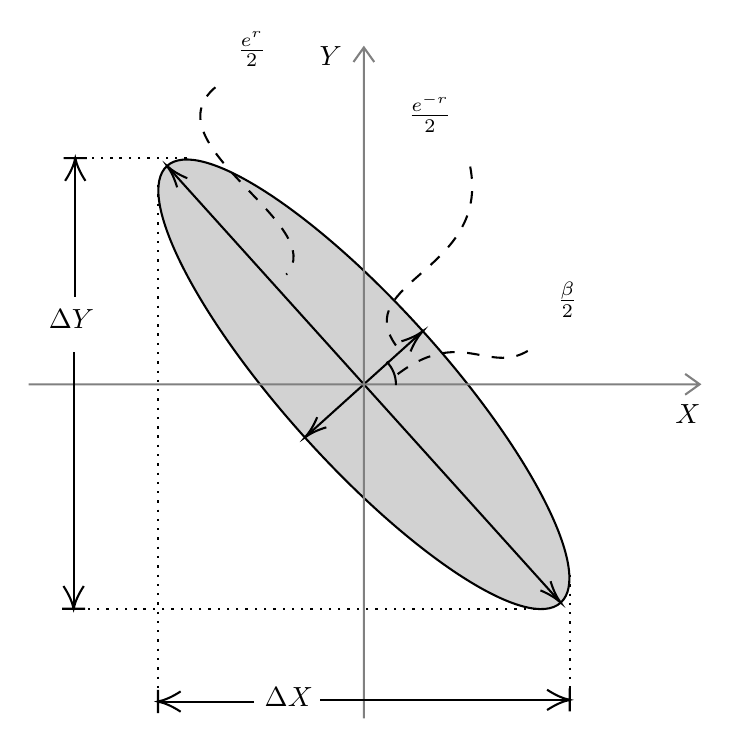
\begin{tikzpicture}[x=0.75pt,y=0.75pt,yscale=-1,xscale=1]
    %uncomment if require: \path (0,467); %set diagram left start at 0, and has height of 467

    %Shape: Ellipse [id:dp8728171396787563] 
    \draw  [color={rgb, 255:red, 0; green, 0; blue, 0 }  ,draw opacity=1 ][fill={rgb, 255:red, 210; green, 210; blue, 210 }  ,fill opacity=1 ] (240.64,132.4) .. controls (256.34,118.25) and (311.51,153.89) .. (363.89,212) .. controls (416.26,270.1) and (446,328.67) .. (430.31,342.82) .. controls (414.61,356.96) and (359.44,321.32) .. (307.06,263.22) .. controls (254.69,205.11) and (224.95,146.54) .. (240.64,132.4) -- cycle ;
    %Straight Lines [id:da7208229415806273] 
    \draw    (428.97,341.33) -- (241.98,133.88) ;
    \draw [shift={(240.64,132.4)}, rotate = 47.97] [color={rgb, 255:red, 0; green, 0; blue, 0 }  ][line width=0.75]    (10.93,-3.29) .. controls (6.95,-1.4) and (3.31,-0.3) .. (0,0) .. controls (3.31,0.3) and (6.95,1.4) .. (10.93,3.29)   ;
    \draw [shift={(430.31,342.82)}, rotate = 227.97] [color={rgb, 255:red, 0; green, 0; blue, 0 }  ][line width=0.75]    (10.93,-3.29) .. controls (6.95,-1.4) and (3.31,-0.3) .. (0,0) .. controls (3.31,0.3) and (6.95,1.4) .. (10.93,3.29)   ;
    %Straight Lines [id:da0649140105673991] 
    \draw    (308.55,261.88) -- (362.4,213.33) ;
    \draw [shift={(363.89,212)}, rotate = 137.97] [color={rgb, 255:red, 0; green, 0; blue, 0 }  ][line width=0.75]    (10.93,-3.29) .. controls (6.95,-1.4) and (3.31,-0.3) .. (0,0) .. controls (3.31,0.3) and (6.95,1.4) .. (10.93,3.29)   ;
    \draw [shift={(307.06,263.22)}, rotate = 317.97] [color={rgb, 255:red, 0; green, 0; blue, 0 }  ][line width=0.75]    (10.93,-3.29) .. controls (6.95,-1.4) and (3.31,-0.3) .. (0,0) .. controls (3.31,0.3) and (6.95,1.4) .. (10.93,3.29)   ;
    %Shape: Axis 2D [id:dp14051364400143518] 
    \draw [color={rgb, 255:red, 128; green, 128; blue, 128 }  ,draw opacity=1 ] (174,237.61) -- (497.27,237.61)(335.47,75.32) -- (335.47,398.59) (490.27,232.61) -- (497.27,237.61) -- (490.27,242.61) (330.47,82.32) -- (335.47,75.32) -- (340.47,82.32)  ;
    %Shape: Arc [id:dp8808247371049068] 
    \draw  [draw opacity=0] (346.44,226.73) .. controls (349.21,229.52) and (350.92,233.36) .. (350.92,237.61) .. controls (350.92,237.72) and (350.92,237.84) .. (350.92,237.95) -- (335.47,237.61) -- cycle ; \draw   (346.44,226.73) .. controls (349.21,229.52) and (350.92,233.36) .. (350.92,237.61) .. controls (350.92,237.72) and (350.92,237.84) .. (350.92,237.95) ;
    %Curve Lines [id:da6027368549559746] 
    \draw  [dash pattern={on 4.5pt off 4.5pt}]  (263.92,94.51) .. controls (231.4,122.15) and (320.03,161.18) .. (298.07,184.76) ;
    %Curve Lines [id:da5486148452364416] 
    \draw  [dash pattern={on 4.5pt off 4.5pt}]  (350.92,218.9) .. controls (328.97,188.01) and (396.45,183.13) .. (386.7,132.72) ;
    %Curve Lines [id:da7051577602263134] 
    \draw  [dash pattern={on 4.5pt off 4.5pt}]  (351.74,232.73) .. controls (384.75,208.01) and (397.27,236.79) .. (419.22,218.09) ;
    %Straight Lines [id:da28339010324533587] 
    \draw  [dash pattern={on 0.84pt off 2.51pt}]  (236.28,141.66) -- (236.28,390.46) ;
    %Straight Lines [id:da6128294010855511] 
    \draw  [dash pattern={on 0.84pt off 2.51pt}]  (434.67,329.48) -- (434.67,390.46) ;
    %Straight Lines [id:da8036441445987096] 
    \draw  [dash pattern={on 0.84pt off 2.51pt}]  (422.47,345.74) -- (196.44,345.74) ;
    %Straight Lines [id:da09093760022431863] 
    \draw  [dash pattern={on 0.84pt off 2.51pt}]  (250.1,128.65) -- (197.25,128.65) ;
    %Straight Lines [id:da6374646769493445] 
    \draw    (196.44,128.65) -- (196.44,195.33) ;
    \draw [shift={(196.44,128.65)}, rotate = 90] [color={rgb, 255:red, 0; green, 0; blue, 0 }  ][line width=0.75]    (0,5.59) -- (0,-5.59)(10.93,-4.9) .. controls (6.95,-2.3) and (3.31,-0.67) .. (0,0) .. controls (3.31,0.67) and (6.95,2.3) .. (10.93,4.9)   ;
    %Straight Lines [id:da8642641164639977] 
    \draw    (282.63,390.46) -- (236.28,390.46) ;
    \draw [shift={(236.28,390.46)}, rotate = 360] [color={rgb, 255:red, 0; green, 0; blue, 0 }  ][line width=0.75]    (0,5.59) -- (0,-5.59)(10.93,-4.9) .. controls (6.95,-2.3) and (3.31,-0.67) .. (0,0) .. controls (3.31,0.67) and (6.95,2.3) .. (10.93,4.9)   ;
    %Straight Lines [id:da433443396267728] 
    \draw    (195.63,222.16) -- (195.63,345.74) ;
    \draw [shift={(195.63,345.74)}, rotate = 270] [color={rgb, 255:red, 0; green, 0; blue, 0 }  ][line width=0.75]    (0,5.59) -- (0,-5.59)(10.93,-4.9) .. controls (6.95,-2.3) and (3.31,-0.67) .. (0,0) .. controls (3.31,0.67) and (6.95,2.3) .. (10.93,4.9)   ;
    %Straight Lines [id:da7910313790713871] 
    \draw    (434.67,389.65) -- (314.34,389.65) ;
    \draw [shift={(434.67,389.65)}, rotate = 180] [color={rgb, 255:red, 0; green, 0; blue, 0 }  ][line width=0.75]    (0,5.59) -- (0,-5.59)(10.93,-4.9) .. controls (6.95,-2.3) and (3.31,-0.67) .. (0,0) .. controls (3.31,0.67) and (6.95,2.3) .. (10.93,4.9)   ;


    % Text Node
    \draw (273.14,66.29) node [anchor=north west][inner sep=0.75pt]    {$\frac{e^{r}}{2}$};
    % Text Node
    \draw (355.42,96.37) node [anchor=north west][inner sep=0.75pt]    {$\frac{e^{-r}}{2}$};
    % Text Node
    \draw (427.18,186.71) node [anchor=north west][inner sep=0.75pt]    {$\frac{\beta }{2}$};
    % Text Node
    \draw (484.1,245.78) node [anchor=north west][inner sep=0.75pt]    {$X$};
    % Text Node
    \draw (312.63,73.41) node [anchor=north west][inner sep=0.75pt]    {$Y$};
    % Text Node
    \draw (182.23,200.25) node [anchor=north west][inner sep=0.75pt]    {$\Delta Y$};
    % Text Node
    \draw (286.21,382.37) node [anchor=north west][inner sep=0.75pt]    {$\Delta X$};


  \end{tikzpicture}


  \caption{Vacío comprimido $\vert z \rangle = \hat{S}(z)\vert 0 \rangle$, con $\beta$ el argumento y $r$ el módulo del parámetro de compresión $z$.}
  \label{fig:squeezed-vacuum}
\end{figure}


En términos de estas amplitudes, el campo eléctrico se puede reescribir como
\begin{equation*}
  \mathbf{E} = i \sum_{k,\lambda} \left( \frac{2\hbar \pi \omega_k}{V} \right)^{1/2} \hat{\mathbf{e}}_{k\lambda} \left[ \hat{Q}\cos(\mathbf{k}\cdot\mathbf{r} - \omega t + \beta) + \hat{P}\sen(\mathbf{k}\cdot\mathbf{r} - \omega t + \beta) \right]
\end{equation*}
De manera más general, un estado comprimido se define por la condición de que existe un ángulo $\beta$ para el cual la dispersión $\langle (\Delta Q)^2 \rangle$ es más pequeño que en el estado vacío, es decir $\langle (\Delta Q)^2 \rangle < 1$. De la relación de incertidumbre se sigue que, necesariamente, $\langle (\Delta P)^2 \rangle > 1$.

En el artículo \textit{Handbuch der Physik} (Pauli, 1933), Wolfgang Pauli desarrolla un método para encontrar los estados de mínima incertidumbre. Esto lo realizó realizando la proposición de que para la función de onda de posición $\varphi(q)$ del estado $\ket{\varphi}$ la cantidad
\begin{equation*}
  \delta = \big| \frac{q }{2\Delta^2 q}\varphi + \frac{\partial \varphi}{\delta p} \big|^2
\end{equation*}
debe ser necesariamente mayor o igual a cero. Desarrollando el binomio e integrando, y usando la definición del operador momento se obtiene
\begin{equation*}
  \int \delta dq = -\frac{1}{4\Delta^2 q} + \Delta^2 p \geq 0
\end{equation*}
que lleva a la relación de incertidumbre de Heisenberg $\Delta q \Delta p \geq \frac{1}{2}$ con $\hbar$ escalada a la unidad. La igualdad se mantiene solo si se satisface
\begin{equation*}
  \frac{1}{2}\frac{q }{\Delta ^2 q} \varphi + \frac{\partial \varphi}{\partial q } = 0
\end{equation*}
la solución normalizada a esta ecuación diferencial es una función de onda Gaussiana, tal como la de un estado coherente
\begin{equation*}
  \varphi(q) = (2\pi\Delta^2q)^{-1/4}\exp{\left( -\frac{q^2}{4\Delta^2 q} \right)}
\end{equation*}
La varianza $\Delta^2 q$ no debe ser necesariamente igual a $1/2$ para mantener la mínima incertidumbre y $\Delta^2 q$ y $\Delta^2 p$ no necesitan ser iguales. $\Delta^2 q$ puede ser menor a $1/2$ dado un $\Delta^2 p$ que mantenga el producto de las incertidumbres fijo en el mínimo. Se parametriza la desviación de las varianzas de los valores del vacío por un número $z$ llamado parámetro de compresión, definiendo
\begin{equation*}
  \Delta^2 q = \frac{1}{2}e^{-2z}, \quad \Delta ^2 p = \frac{1}{2}e^{2z}
\end{equation*}
Para comprimir el vacío, se puede escalar la funcion de onda $\psi_0$
\begin{equation*}
  \varphi(q) = e^{z/2}\psi_0(e^{-z}p)
\end{equation*}
donde la función ya está normalizada. La función de onda del momento $\tilde{\varphi}(p)$ es la transformada de Fourier de la función de onda de la posición
\begin{equation*}
  \tilde{\varphi}(p) = e^{-z/2}\tilde{\psi}_0(e^{-z}p)
\end{equation*}
De las anteriores dos ecuaciones de puede observar que, cuando la función de onda de la posición se ve comprimida, la de momento se estira y viceversa. Diferenciando la función de onda de posición respecto al parámetro de compresión se obtiene \cite{Leonhardt}
\begin{equation*}
  \frac{\partial \varphi}{\partial z} = \frac{1}{2}\left( i\hat{q}\hat{p} + i\hat{p}\hat{q} \right)\varphi = \frac{1}{2}\left( {\hat{a}}^2 - {\hat{a}^{\dagger}}^2 \right)\varphi
\end{equation*}
La solución entonces se puede expresar en términos del operador de compresión, definido como
\begin{equation*}
  \hat{S}(z) = \exp{\left( \frac{z}{2}(\hat{a}^2 - {\hat{a}^{\dagger}}^2) \right)}
\end{equation*}
del estado vacío se obtiene entonces
\begin{equation*}
  \ket{\varphi} = \hat{S}(z)\ket{0}
\end{equation*}
Esta definición del operador compresión permite comprimir al estado vacío solo a lo largo y ancho de los ejes del espacio fase, sin embargo, como se discutió al inicio del capítulo, un estado comprimido puede rotar un ángulo $\beta$ en el espacio fase, y la elipse que representa al estados no necesariamente tiene su semieje mayor o menor en paralelo con los ejes del espacio fase. La forma más general del operador de compresión como operador unitario considera al argumento del parámetro de compresión $z$ como complejo, lo que permite que la compresión se de respecto a otro eje no necesariamente paralelo al de la cuadratura de momento o posición \cite{Loudon}
\begin{equation*}
  \hat{S}(z) = \exp{\left( \frac{1}{2} (z{\hat{a}^{\dagger}}^2 - z^* {\hat{a}}^2) \right)}, \quad z = re^{i\beta}
\end{equation*}

Del teorema de expansión de operadores, se puede encontrar la transformación unitaria del operador aniquilación $\hat{a}$ por el de compresión $\hat{S}(z)$,
\begin{align*}
  \hat{A}(z) & = \hat{S}(z)\hat{a} \hat{S}(z)                                                                       \\
             & = \hat{a}  + z\hat{a}^{\dagger} + \frac{|z|^2\hat{a}}{2!} + \frac{z|z|^2\hat{a}^{\dagger}}{3!}+\dots \\
             & = \hat{a} \cosh{r} + \hat{a}^{\dagger} e^{i\beta}\senh{r}                                            \\
             & = \mu\hat{a} + \nu\hat{a}^{\dagger}
\end{align*}
donde se ha definido $\mu = \cosh{r}$ y $\nu = e^{i\beta}\senh{r}$. De manera análoga se obtiene la transformación unitaria del operador creación
\begin{align*}
  \hat{A}^{\dagger}(z) & = \hat{S}(z)\hat{a}^{\dagger} \hat{S}(z) \\
                       & = \mu\hat{a} + \nu^* \hat{a}
\end{align*}
Los operadores $\hat{A}(z)$ y $\hat{A}^\dagger(z)$ siguen la misma relación de conmutación que los operadores escalera
\begin{equation*}
  [\hat{A}, \hat{A}^{\dagger})] = 1
\end{equation*}
donde se deja implícita la dependencia de estos operadores en el parámetro de compresión $z$. La relación entre estos operadores y los de escalera está dada por
\begin{align*}
  \hat{a}           & = \mu \hat{A} - \nu \hat{A}^\dagger   \\
  \hat{a}^{\dagger} & = \mu \hat{A}^\dagger - \nu^* \hat{A}
\end{align*}

El estado que se obtiene al aplicar el operador de compresión en un estado coherente $\ket{\alpha}$ se denomina estado coherente de dos fotones \cite{Mandel}, denotado por
\begin{equation*}
  \ket{[z,\alpha]} = \hat{S}(z)\ket{\alpha} = \hat{S}(z)\hat{D}(\alpha)\ket{0}
\end{equation*}
Dado que los operadores compresión y desplazamiento no conmutan, se puede definir también el estado compresión ideal, invirtiendo el orden de los operadores sobre el estado vacío \cite{Loudon}
\begin{equation*}
  \ket{\alpha, z} = \hat{D}(\alpha) \hat{S}(z) \ket{0}
\end{equation*}
Los valores esperados de para los estados coherentes comprimidos están dados por
\begin{align*}
  \hat{S}^\dagger(z) \hat{D}^\dagger (\alpha) \hat{a} \hat{S}(z) \hat{D}(\alpha)           & = \hat{a} \cosh{r} - \hat{a}^{\dagger} e^{i\theta}\senh{r}             \\ \alpha
  \hat{S}^\dagger(z) \hat{D}^\dagger (\alpha) \hat{a}^{\dagger} \hat{S}(z) \hat{D}(\alpha) & = \hat{a}^{\dagger} \cosh{r} - \hat{a} e^{-i\theta}\senh{r} + \alpha^*
\end{align*}
de estas transformaciones, se puede obtener una relación de eigenvalores para los estados coherentes comprimidos
\begin{equation*}
  \left( \hat{a} \cosh{r} + \hat{a}^{\dagger} e^{i\theta} \senh{r} \right) \ket{\alpha, z} = \left( \alpha \cosh{r} + \alpha^* e^{i\theta} \senh{r} \right) \ket{\alpha, z}
\end{equation*}
El principal interés del estudio de los estados coherentes comprimidos radica en las propiedades de los operadores cuadraturas relacionados a estos, se tiene que
\begin{align*}
  \bra{\alpha, z}\hat{X}\ket{\alpha, z}   & = \Re \alpha & = |\alpha| \cos\phi \\
  \bra{\alpha, z} \hat{Y} \ket{\alpha, z} & = \Im \alpha & = |\alpha| \sen\phi
\end{align*}
donde $\alpha = |\alpha|e^{i\phi}$. Las varianzas en las cuadraturas son
\begin{align*}
  (\Delta X)^2 & = \frac{1}{4}\left( e^{2r}\sen^2{\left( \frac{\theta}{2} \right)} +e^{-2r}\cos^2{\left( \frac{\theta}{2} \right)} \right) \\
  (\Delta Y)^2 & = \frac{1}{4}\left( e^{2r}\cos^2{\left( \frac{\theta}{2} \right)} +e^{-2r}\sen^2{\left( \frac{\theta}{2} \right)} \right)
\end{align*}
(Rehacer figura 5.10 Loudon con descripción de los operadores en la cuadratura)

El operador de tiene la siguiente propiedad
\begin{equation*}
  \hat{S}^{\dagger}(z) = \hat{S}^{-1}(z) = \hat{S}(-z)
\end{equation*}
Escribiendo el operador de aniquilación como la combinación de dos operadores hermitianos $\hat{X}$ y $\hat{Y}$ como se realizó en la sección del oscilador armónico, se encontró que su relación de incertidumbre es $\Delta X \Delta Y \leq 1/4$ y los estados coherentes tienen la particularidad de tener los estados de menor incertidumbre, es decir, cumplen el caso de la igualdad y $\Delta X = \Delta Y = \frac{1}{2}$. Dependiendo de cómo se definan estos operadores Hermitianos en los que se descomponen los operadores de aniquilación y creación, se escalan estos en el espacio de fasores. (Agregar cómo lo define Wals, Agarwal y otros para denotar las diferencias y especificar que se usa la definición de Loudon)
(Walls, Milburn)

\begin{figure}[!h]
  \centering


  \tikzset{every picture/.style={line width=0.75pt}} %set default line width to 0.75pt        

  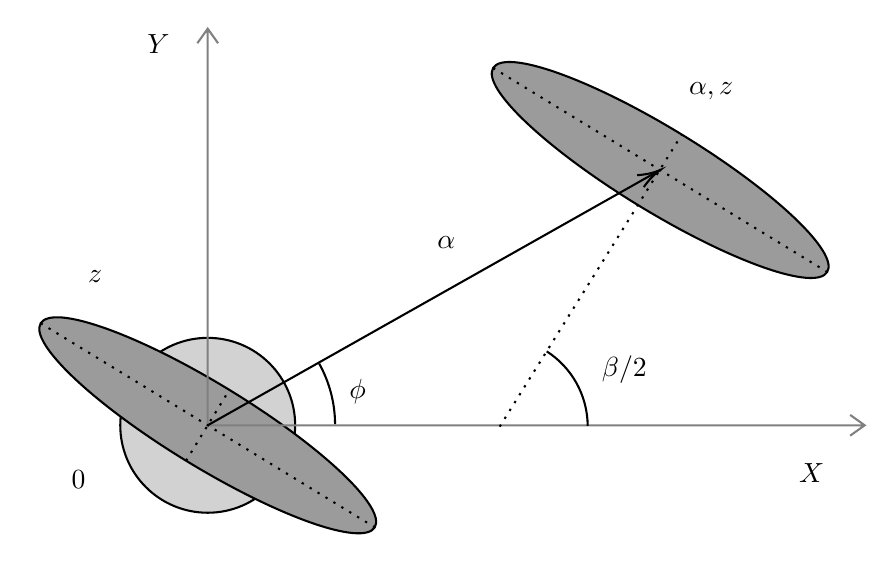
\begin{tikzpicture}[x=0.75pt,y=0.75pt,yscale=-1,xscale=1]
    %uncomment if require: \path (0,454); %set diagram left start at 0, and has height of 454

    %Shape: Circle [id:dp9937485135549077] 
    \draw  [fill={rgb, 255:red, 210; green, 210; blue, 210 }  ,fill opacity=1 ] (169.47,281.6) .. controls (169.47,258.33) and (188.33,239.47) .. (211.6,239.47) .. controls (234.87,239.47) and (253.73,258.33) .. (253.73,281.6) .. controls (253.73,304.87) and (234.87,323.73) .. (211.6,323.73) .. controls (188.33,323.73) and (169.47,304.87) .. (169.47,281.6) -- cycle ;
    %Shape: Ellipse [id:dp23338310549536545] 
    \draw  [fill={rgb, 255:red, 155; green, 155; blue, 155 }  ,fill opacity=1 ] (292.08,330.75) .. controls (286.32,340.17) and (245.63,325.81) .. (201.18,298.67) .. controls (156.73,271.53) and (125.36,241.88) .. (131.12,232.45) .. controls (136.88,223.03) and (177.57,237.39) .. (222.02,264.53) .. controls (266.47,291.67) and (297.84,321.32) .. (292.08,330.75) -- cycle ;
    %Shape: Ellipse [id:dp9660486804123943] 
    \draw  [fill={rgb, 255:red, 155; green, 155; blue, 155 }  ,fill opacity=1 ] (510.08,207.75) .. controls (504.32,217.17) and (463.63,202.81) .. (419.18,175.67) .. controls (374.73,148.53) and (343.36,118.88) .. (349.12,109.45) .. controls (354.88,100.03) and (395.57,114.39) .. (440.02,141.53) .. controls (484.47,168.67) and (515.84,198.32) .. (510.08,207.75) -- cycle ;
    %Shape: Axis 2D [id:dp27291625147732324] 
    \draw [color={rgb, 255:red, 128; green, 128; blue, 128 }  ,draw opacity=1 ] (211.6,281.6) -- (528.13,281.6)(211.6,90.53) -- (211.6,281.6) -- cycle (521.13,276.6) -- (528.13,281.6) -- (521.13,286.6) (206.6,97.53) -- (211.6,90.53) -- (216.6,97.53)  ;
    %Straight Lines [id:da03545042046202651] 
    \draw  [dash pattern={on 0.84pt off 2.51pt}]  (349.12,109.45) -- (510.08,207.75) ;
    %Straight Lines [id:da32039076300728264] 
    \draw  [dash pattern={on 0.84pt off 2.51pt}]  (131.12,232.45) -- (292.08,330.75) ;
    %Shape: Arc [id:dp6895361690264035] 
    \draw  [draw opacity=0] (265.3,251.87) .. controls (270.11,260.53) and (272.88,270.48) .. (272.97,281.06) -- (211.6,281.6) -- cycle ; \draw   (265.3,251.87) .. controls (270.11,260.53) and (272.88,270.48) .. (272.97,281.06) ;
    %Shape: Arc [id:dp5481123255537238] 
    \draw  [draw opacity=0] (374.94,245.99) .. controls (386.71,253.53) and (394.55,266.78) .. (394.68,281.88) -- (352.28,282.25) -- cycle ; \draw    (374.94,245.99) .. controls (386.71,253.53) and (394.55,266.78) .. (394.68,281.88) ;
    %Straight Lines [id:da36293450996765164] 
    \draw [color={rgb, 255:red, 0; green, 0; blue, 0 }  ,draw opacity=1 ]   (211.6,281.6) -- (427.86,159.58) ;
    \draw [shift={(429.6,158.6)}, rotate = 150.57] [color={rgb, 255:red, 0; green, 0; blue, 0 }  ,draw opacity=1 ][line width=0.75]    (10.93,-3.29) .. controls (6.95,-1.4) and (3.31,-0.3) .. (0,0) .. controls (3.31,0.3) and (6.95,1.4) .. (10.93,3.29)   ;
    %Straight Lines [id:da0816848118648823] 
    \draw  [dash pattern={on 0.84pt off 2.51pt}]  (201.18,298.67) -- (222.02,264.53) ;
    %Straight Lines [id:da23379922428710298] 
    \draw  [dash pattern={on 0.84pt off 2.51pt}]  (352.28,282.25) -- (440.02,141.53) ;

    % Text Node
    \draw (495,298.4) node [anchor=north west][inner sep=0.75pt]    {$X$};
    % Text Node
    \draw (181,92.07) node [anchor=north west][inner sep=0.75pt]    {$Y$};
    % Text Node
    \draw (320.7,188.97) node [anchor=north west][inner sep=0.75pt]    {$\alpha $};
    % Text Node
    \draw (400.03,246.73) node [anchor=north west][inner sep=0.75pt]    {$\beta /2$};
    % Text Node
    \draw (278.33,257.73) node [anchor=north west][inner sep=0.75pt]    {$\phi $};
    % Text Node
    \draw (144.5,301.8) node [anchor=north west][inner sep=0.75pt]    {$\ket{0}$};
    % Text Node
    \draw (152.5,205.8) node [anchor=north west][inner sep=0.75pt]    {$\ket{z}$};
    % Text Node
    \draw (442,114.8) node [anchor=north west][inner sep=0.75pt]    {$\ket{\alpha ,z}$};


  \end{tikzpicture}


  \caption{Estado comprimido ideal, donde se aplica primero la compresión y después el desplazamiento sobre el estado vacío $\vert\alpha, z\rangle = \hat{D}(\alpha)\hat{S}(z)\vert0\rangle$, con $\beta$ la fase del parámetro de compresión $z$, $\alpha$ el parámetro de desplazamiento y $\phi$ el argumento de desplazamiento}
  \label{fig:disp-squeezed-state}
\end{figure}
